\chapter{结果讨论与分析}
本章将对搭建的骨关节炎风险预测模型的图估计效果、患病风险预测能力进行分析与评估。同时将结合具体案例分析模型解释器所产生的解释结果。
\section{评估指标}
为了对模型的风险预测能力进行科学的评估,本文依照真实样本标签与预测结果构建如下混淆矩阵(Confusion Matrix)并根据该矩阵计算常用评价指标\cite{gaudillo_machine_2019}
\begin{table}[!h]
	\renewcommand{\arraystretch}{1.2}
	\centering\wuhao
	\caption{混淆矩阵相关指标} \label{ICD_exclude} \vspace{2mm}
	\begin{tabularx}{\textwidth} { 
   >{\centering\arraybackslash}X 
   >{\centering\arraybackslash}X
   >{\centering\arraybackslash}X}
	\toprule[1.5pt]
		指标 & 计算公式 & 含义 \\
	\midrule[1pt]
		准确率 Accuracy & $\frac{TP+TN}{TP+TN+FP+FN}$ & 模型整体判断准确程度 \\
        召回率 Recall & $\frac{TP}{TP+FN}$ &
        正确预测阳性样本占总阳性样本的比例 \\
        特异度 Specificity & $\frac{TN}{TN+FP}$ &
        正确预测阴性样本占总阴性样本的比例 \\
        精确度 Precision & $\frac{TP}{TP+FP}$ &
        正确预测阳性样本占预测结果为真的样本比例 \\
        F1分数 & $\frac{2*Precision*Recall}{Precision+recall}$ &
        综合召回率与精确度评估模型预测准确程度 \\
	\bottomrule[1.5pt]
	\end{tabularx}
\end{table}
此外,在评估模型预测效果时还有另一种不依赖混淆矩阵的指标,本文使用了其中的两种——接收器操作特性曲线下面积(Area Under Receiver Operating Curve,AUROC)以及柯尔莫哥洛夫-斯米尔诺夫指标(Kolmogorov-Smirnov Statistic,K-S Statistic)。接收器操作特性曲线(ROC)是用来评价二元分类器分类能力的一种曲线,其以真阳性率为纵轴假阳性率为横轴绘制模型不同阈值下真假阳性率的坐标。其曲线与横轴所围成面积被称为曲线下面积(AUC),对于一分类模型而言,AUC越高表示其做出正确判断的能力越强。\cite{fawcett_introduction_2006}并且同准确率相比,AUC评价时不受训练集正负样本比例所影响。\cite{zou_receiver-operating_2007}因此本文使用该指标衡量模型预测能力。具有相似功能的指标还有K-S\cite{naaman_tight_2021},它是一种用来检验两经验分布之间是否相同的统计量,K-S量越大表明模型的区分能力越强。
\section{模型预测效果评价}
\subsection{基准计算}
在对本模型效果进行分析前,我们首先需要计算使用传统PRS方法时骨关节炎的风险预测效果。PRS方法,又称多基因风险评分(Polygenetic Risk Score)方法\cite{dudbridge_power_2013},是一种评估SNP位点对某一特定性状的累计影响的量化指标。它由已有GWAS研究结果中SNP对表型影响的效应值以及统计显著性构建。其计算公式为
\begin{equation}
    S=\sum_i^N X_i \beta_i
\end{equation}

其中$S$为个体的风险评分,$N$为总潜在SNP的数量,$X_i$为第$i$个SNP中潜在效应等位基因的数量,$\beta_i$为第$i$个SNP对形状的效应值。我们根据该公式对现有基因型数据进行计算得到个体评分,再通过逻辑回归法构建基于PRS的风险预测模型并得到如下ROC曲线

可以发现,传统PRS模型的风险预测效果较差,AUC仅为0.51,与随机预测相当。这意味着使用PRS模型对骨关节炎的预测几乎没有任何参考意义。这也与Boer[5]研究中构建的PRS模型结果相符。同时我们也使用了包括决策树算法在内额若干传统机器学习模型对基因型数据进行处理与预测,所得结果与基于PRS的模型无显著差异。本文因此以该PRS模型为基础讨论本文提出模型对预测效果的改善。
\begin{table}[!h]
	\renewcommand{\arraystretch}{1.2}
	\centering\wuhao
	\caption{混淆矩阵相关指标} \label{ICD_exclude} \vspace{2mm}
	\begin{tabularx}{\textwidth} { 
   >{\centering\arraybackslash}X 
   >{\centering\arraybackslash}X
   >{\centering\arraybackslash}X}
	\toprule[1.5pt]
		指标 & 基于PRS的模型 & 决策树模型 \\
	\midrule[1pt]
		auc & 0.51 & 0.50 \\
        f1 & 0.45 & 0.29 \\
        accuracy & 0.52 & 0.51 \\
        precision & 0.50 & 0.50 \\
        recall & 0.41 & 0.21 \\
	\bottomrule[1.5pt]
	\end{tabularx}
\end{table}

\begin{figure}[!ht]
\centering
\subfigure[PRS模型的ROC曲线]{
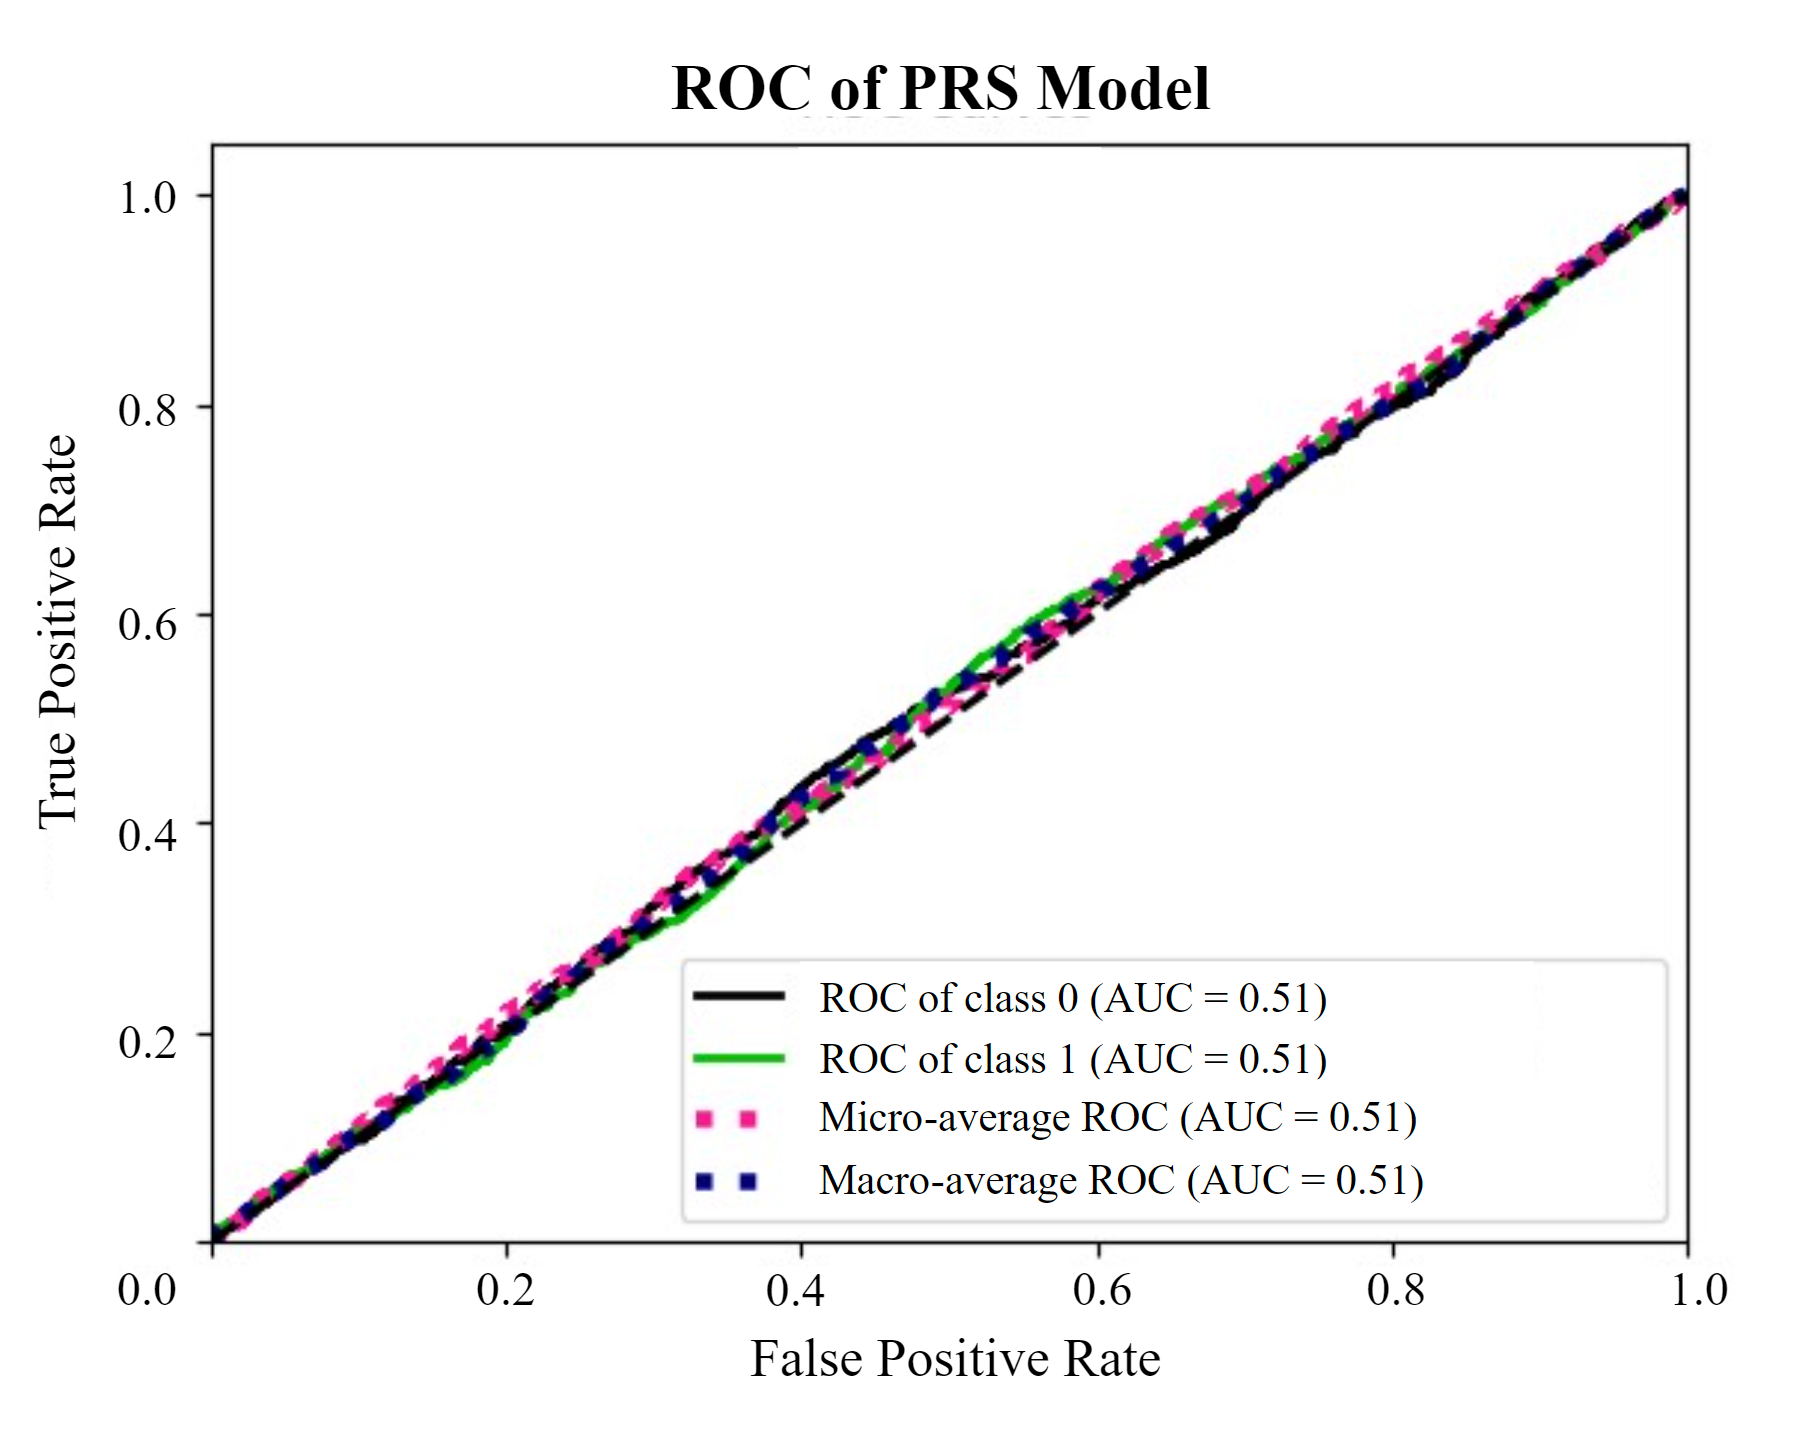
\includegraphics[width=7cm]{figures/Chapter4/GNN/PRSROC.png}
}
\subfigure[决策树模型的ROC曲线]{
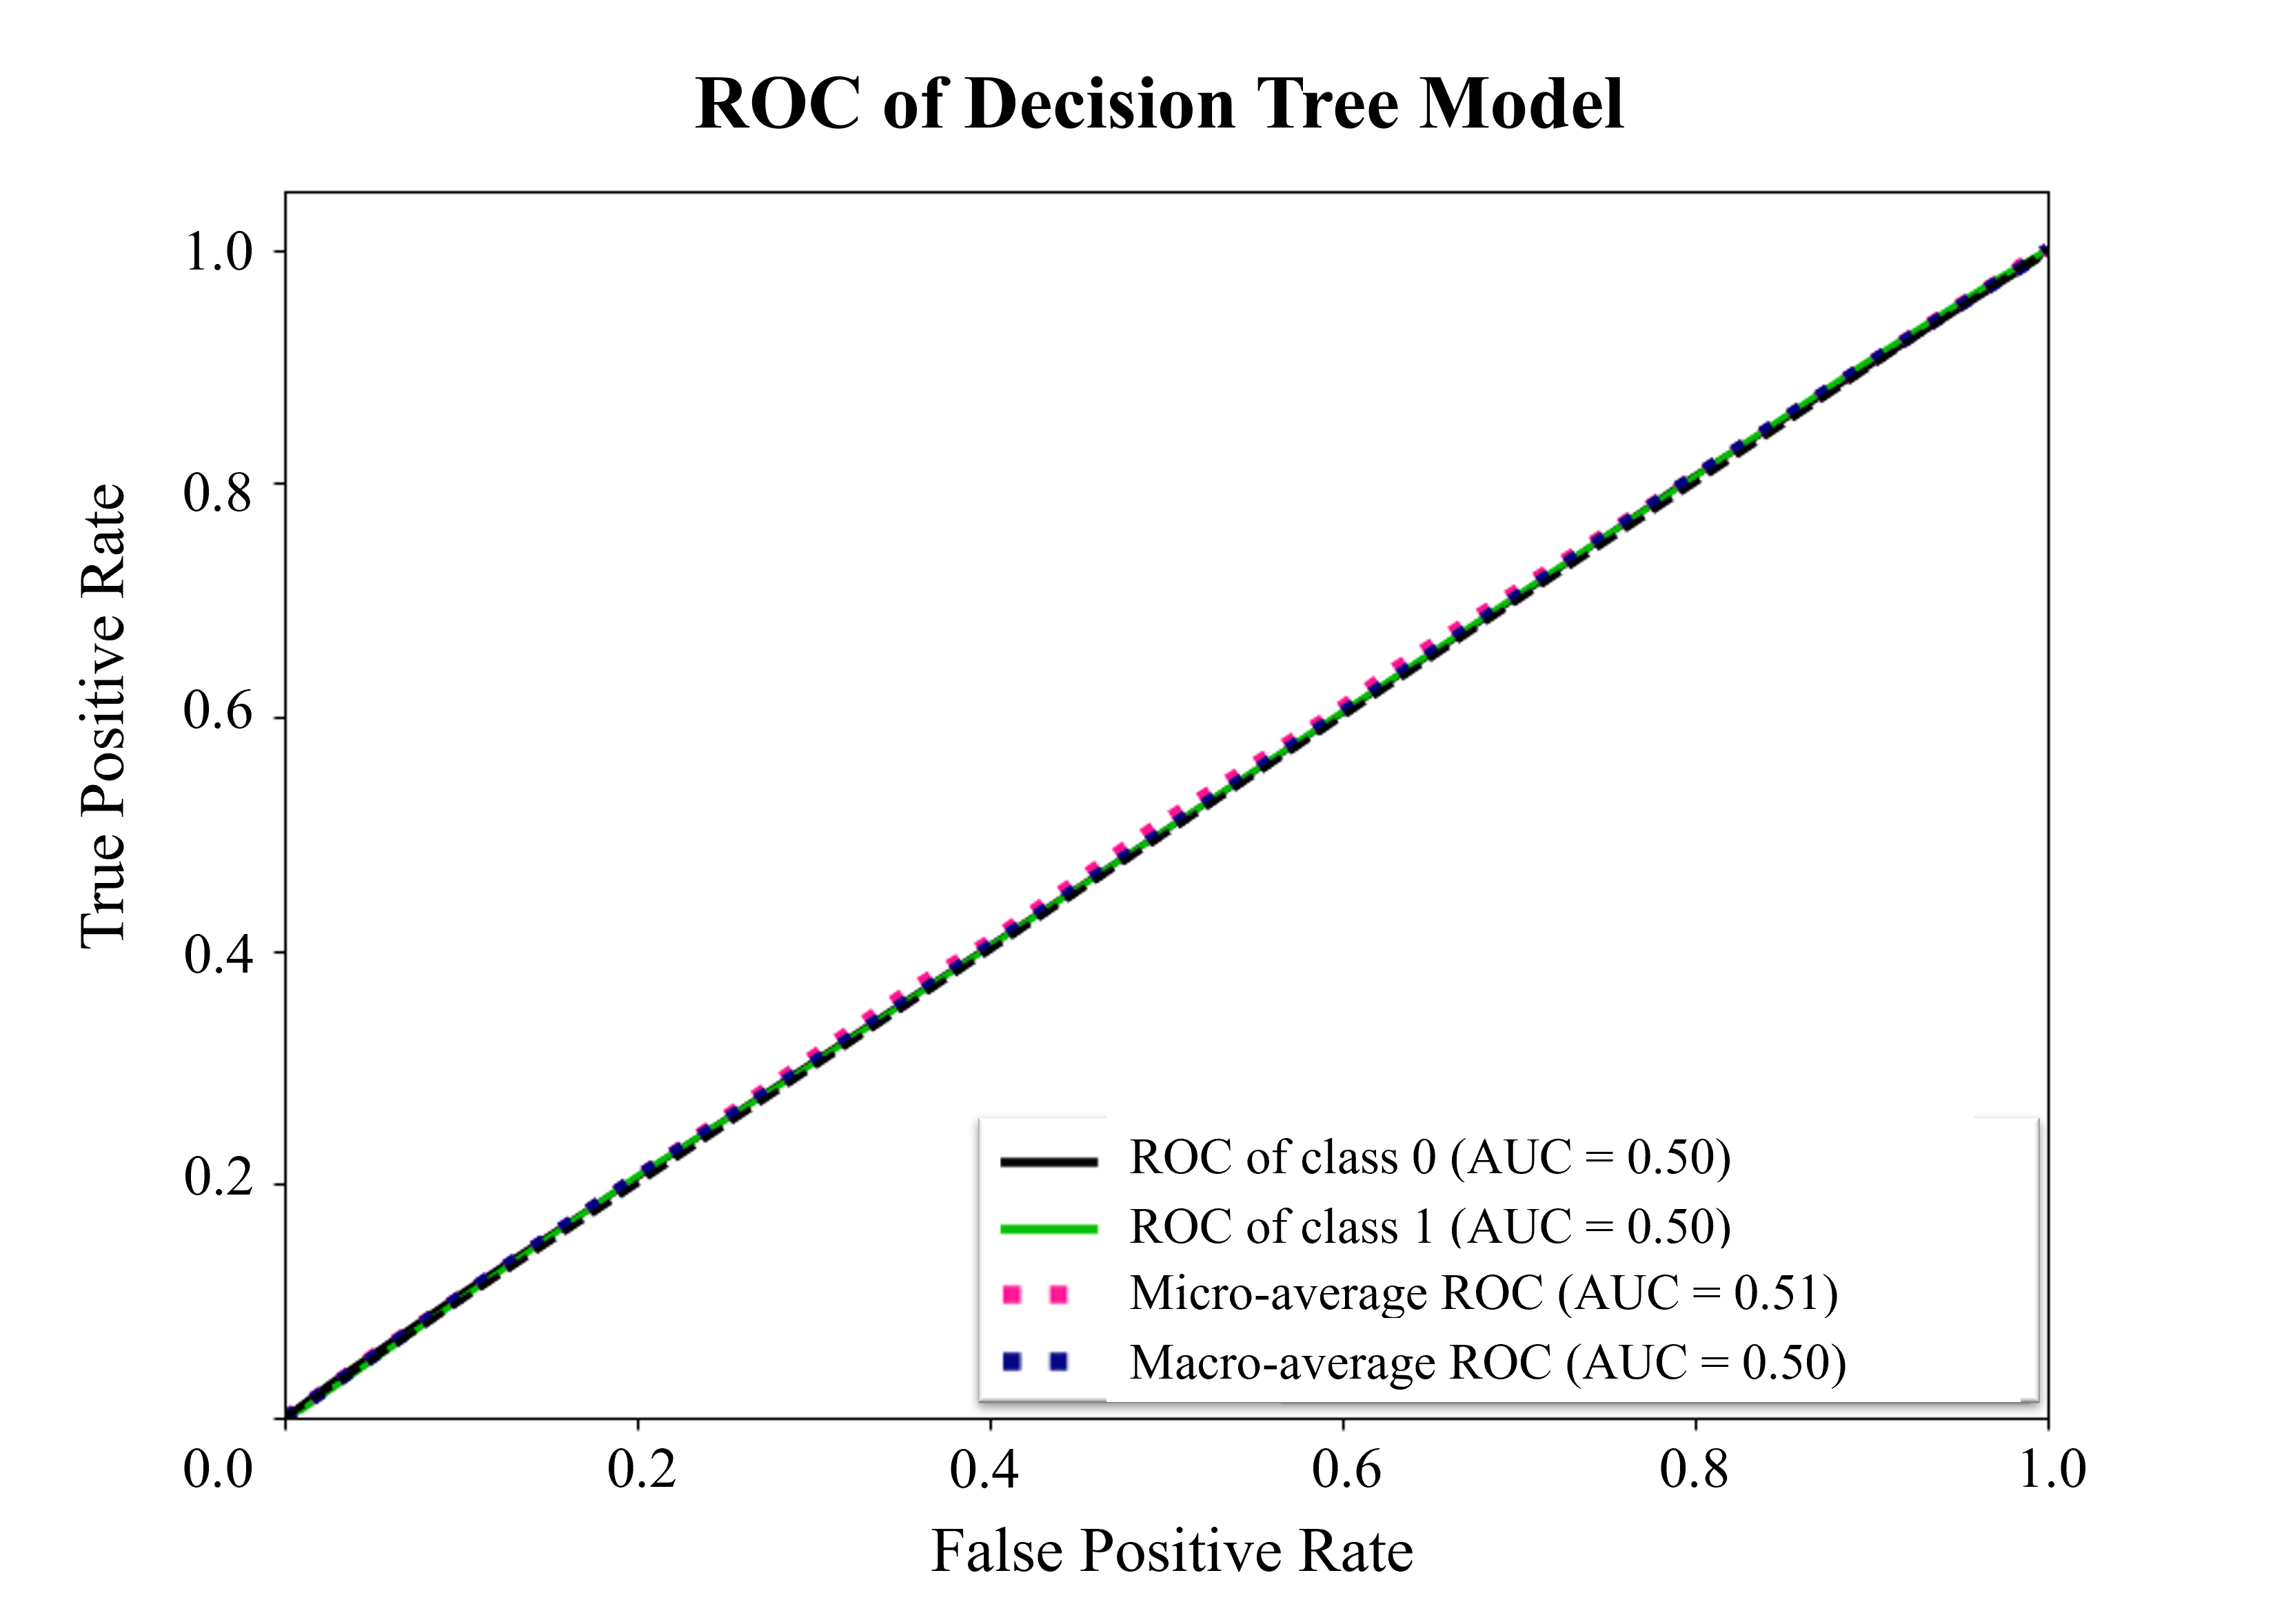
\includegraphics[width=7.5cm]{figures/Chapter4/GNN/DTROC.png}
}
\caption{基准模型ROC曲线}
\end{figure}



\subsection{特征筛选方法对比}
之前的讨论中我们提到,特征筛选对于特征数与样本数之比较高的数据集有着很好的提高模型性能的效果。本文也因此提到了两种特征筛选方法——基于卡方的样本筛选与基于支持向量机的样本筛选。对于使用同样超参数的决策树模型,我们输入使用不同特征筛选方式处理后的数据集并比较两种特征筛选方法对模型效果的影响。结果如下表。

\begin{table}[!h]
	\renewcommand{\arraystretch}{1.2}
	\centering\wuhao
	\caption{特征筛选方法对比} \label{ICD_exclude} \vspace{2mm}
	\begin{tabularx}{\textwidth} { 
   >{\centering\arraybackslash}X 
   >{\centering\arraybackslash}X
   >{\centering\arraybackslash}X}
	\toprule[1.5pt]
	指标 & 经卡方法筛选特征 & 经支持向量机法筛选特征 \\
	\midrule[1pt]
	auc & 0.51 & 0.54 \\
f1 & 0.38 & 0.43 \\
accuracy & 0.52 & 0.54 \\
precision & 0.51 & 0.55 \\
recall & 0.29 & 0.35 \\
	\bottomrule[1.5pt]
	\end{tabularx}
\end{table}
\begin{figure}[htbp]
\centering
\subfigure[使用卡方法筛选后模型ROC曲线]{
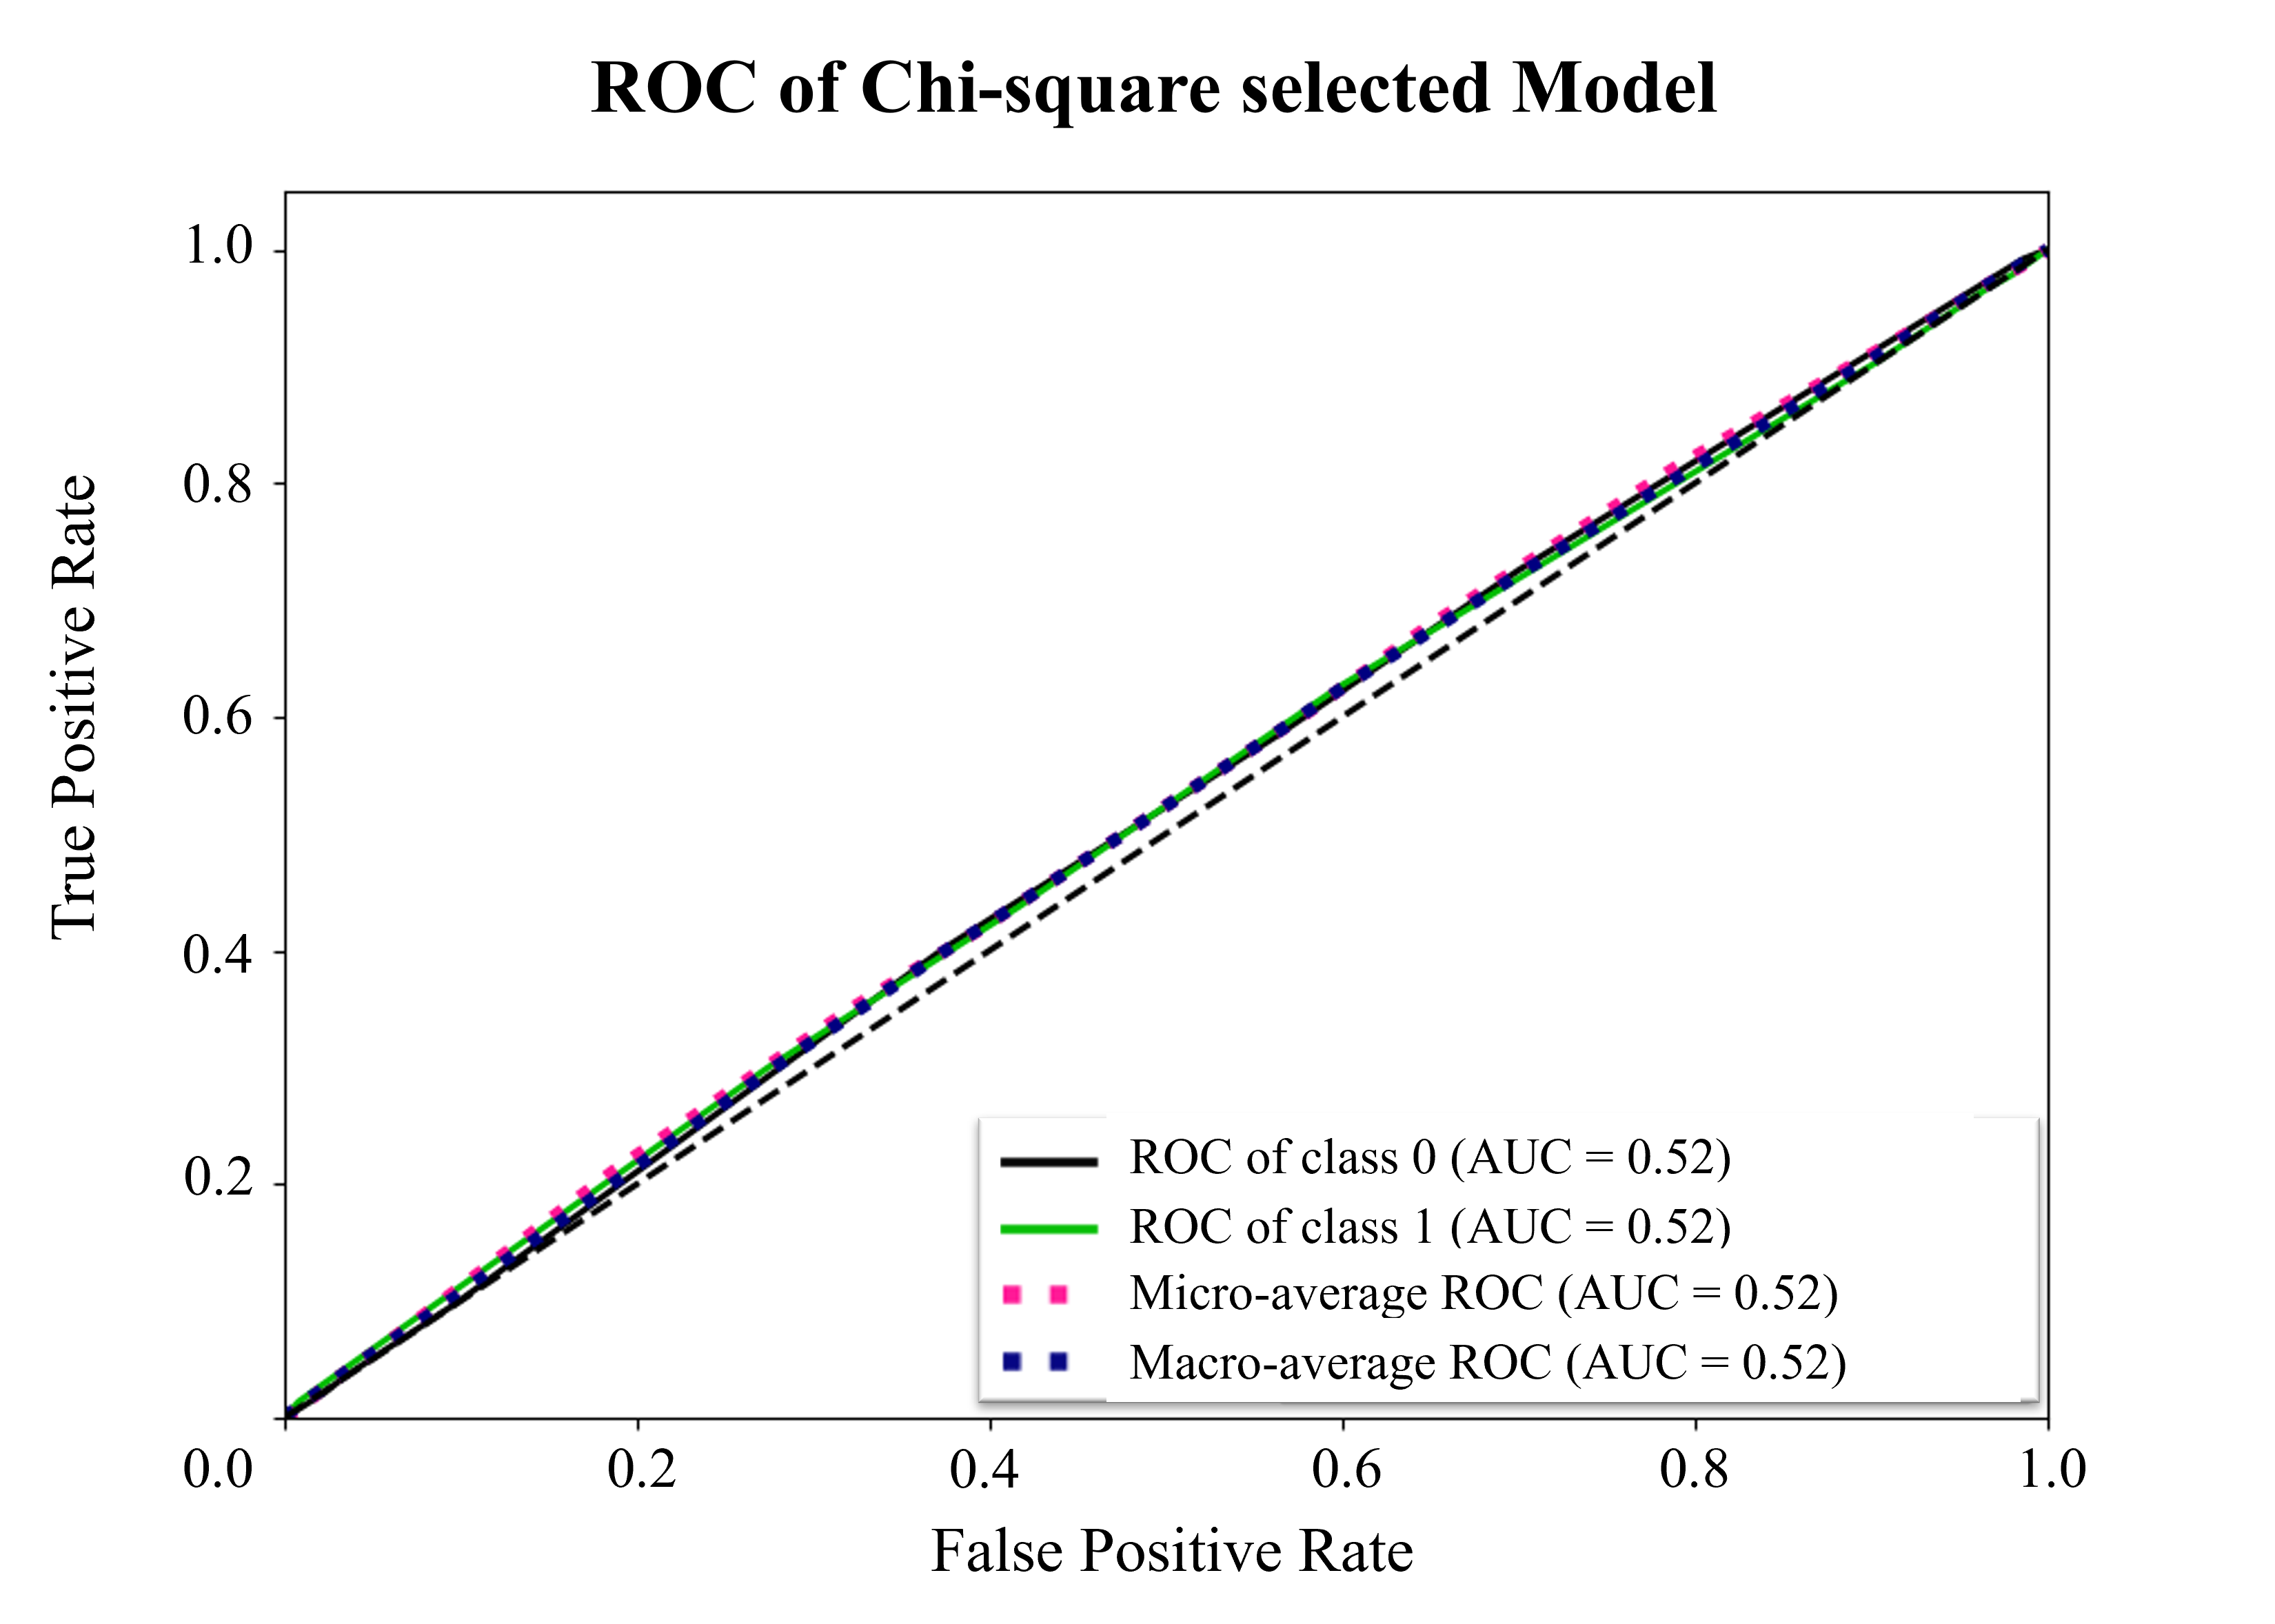
\includegraphics[width=7cm]{figures/Chapter4/GNN/CSROC.png}
}
\quad
\subfigure[使用卡方法筛选后模型KS曲线]{
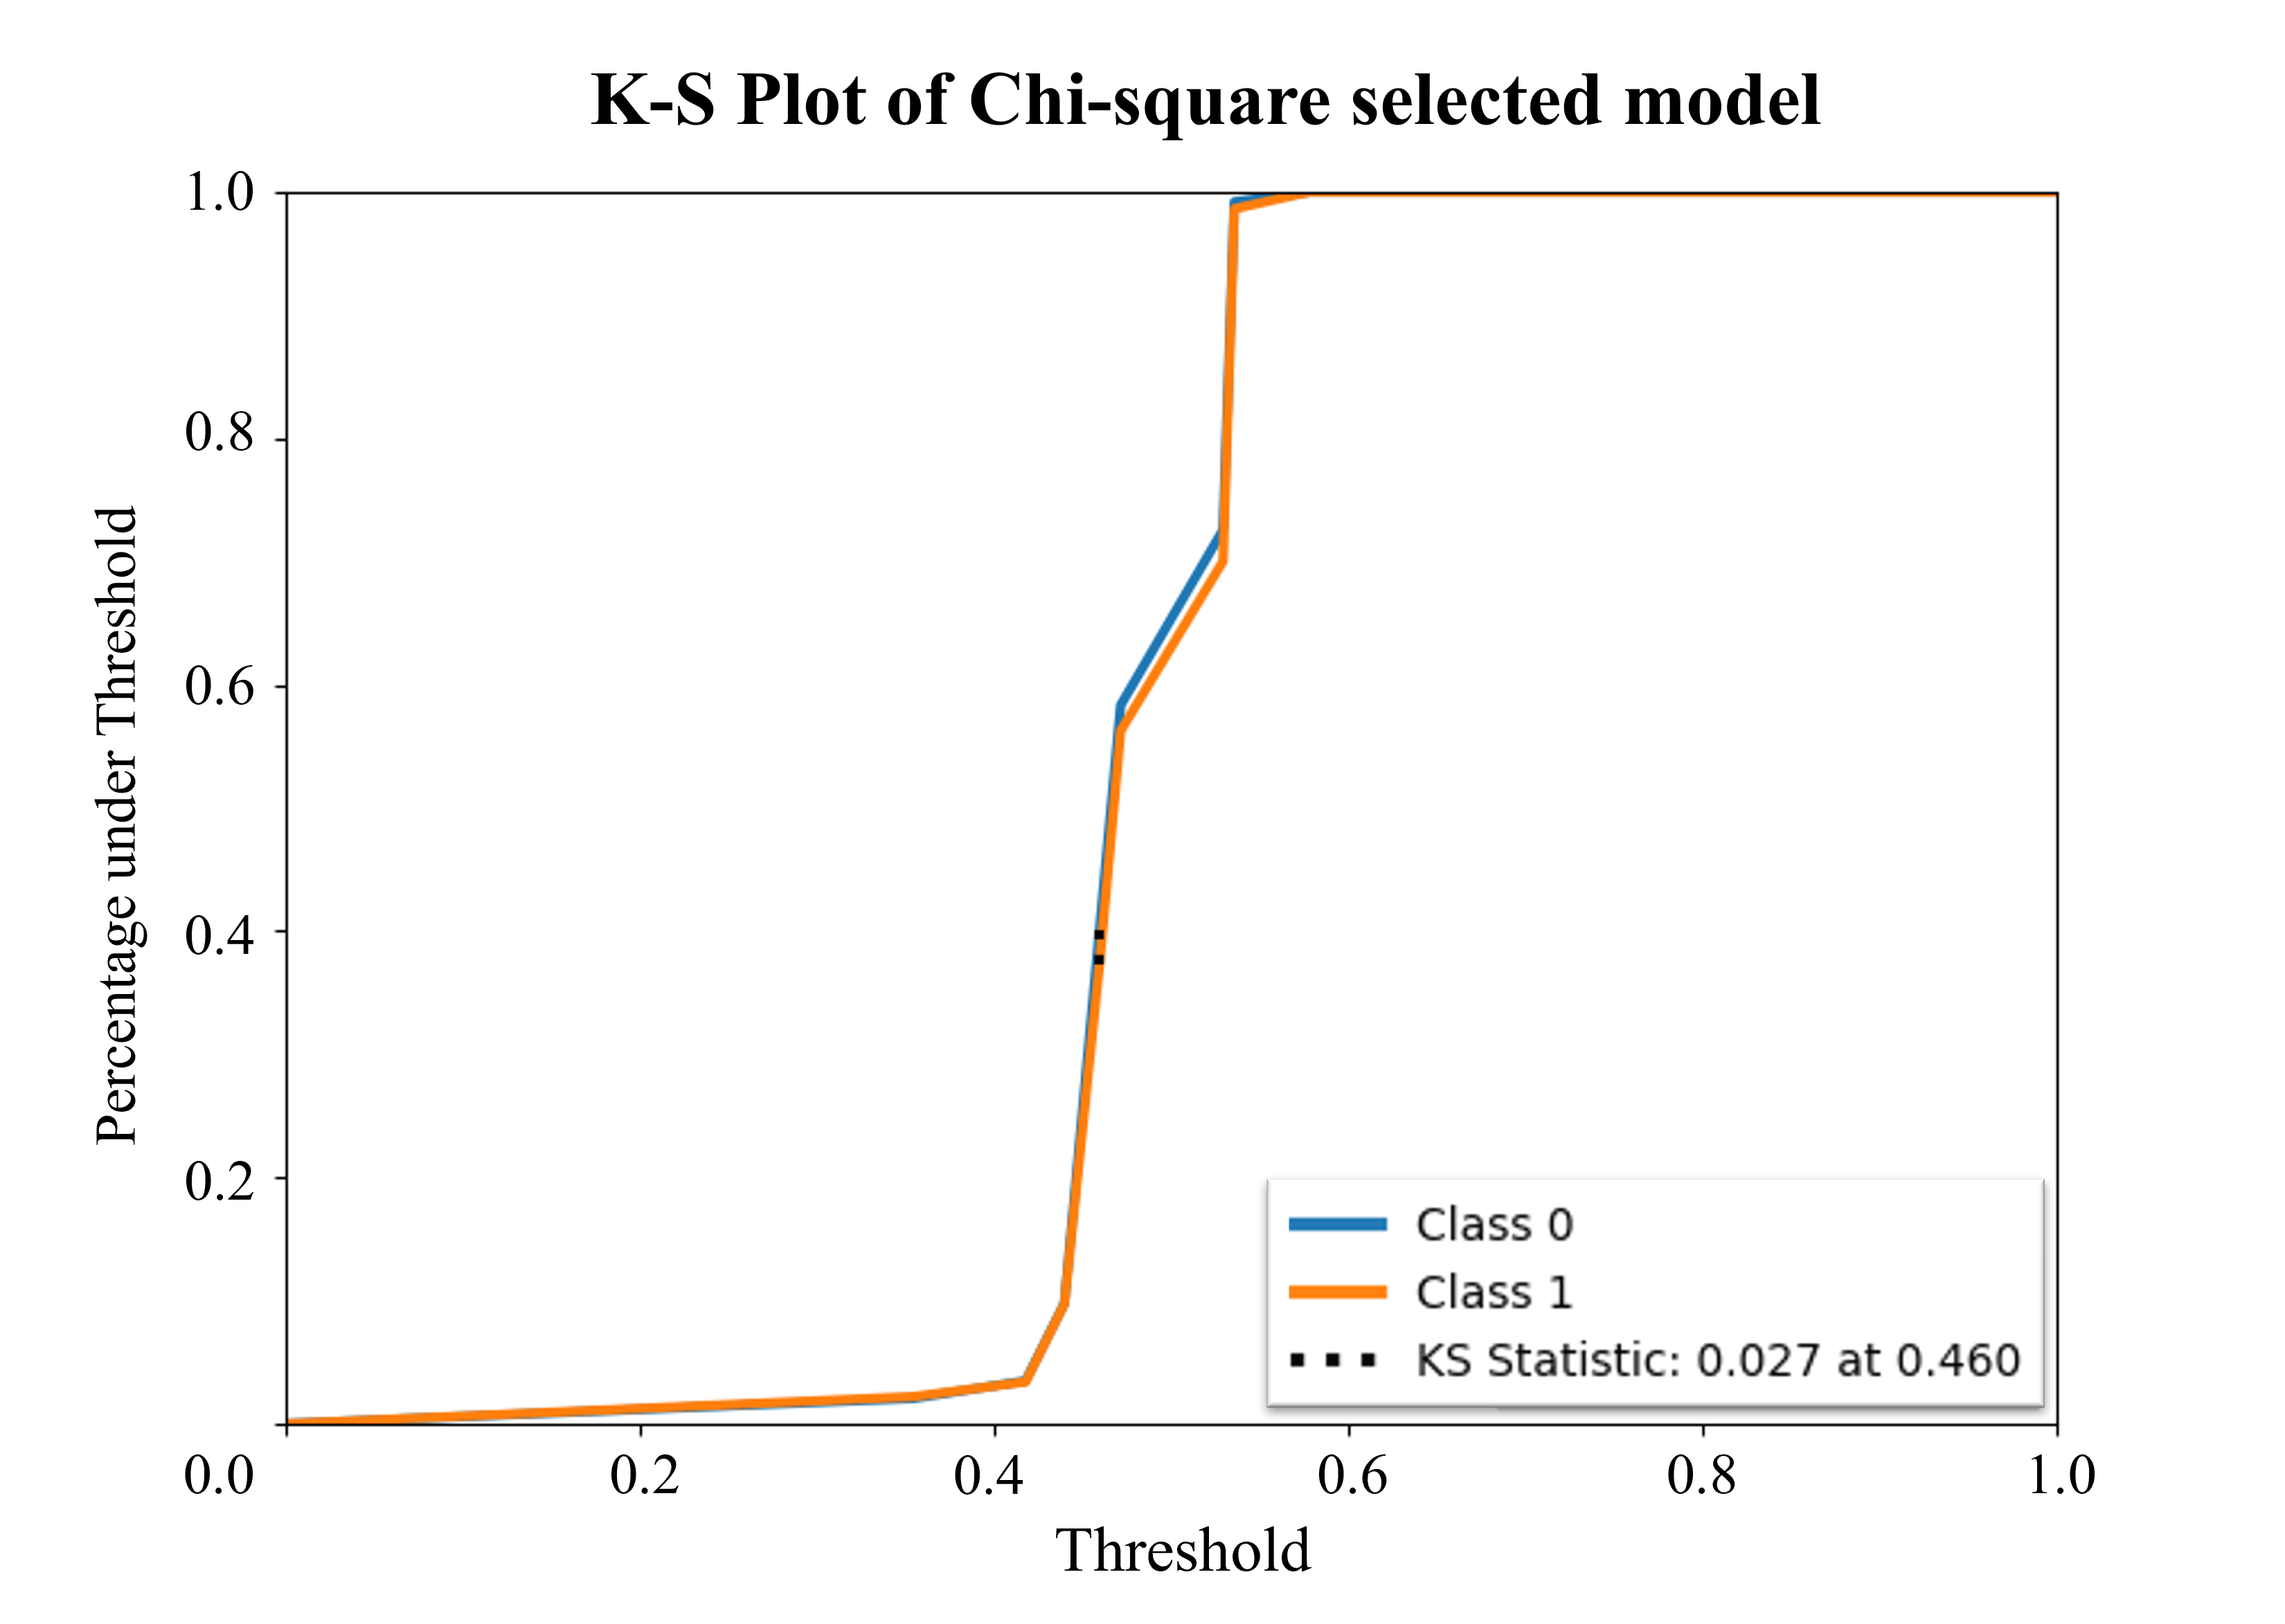
\includegraphics[width=7cm]{figures/Chapter4/GNN/CSKS.png}
}
\quad
\subfigure[使用支持向量机法筛选后模型ROC曲线]{
\includegraphics[width=7cm]{figures/Chapter4/GNN/SVCROC.png}
}
\quad
\subfigure[使用支持向量机法筛选后模型KS曲线]{
\includegraphics[width=7cm]{figures/Chapter4/GNN/SVCKS.png}
}
\caption{不同方法特征筛选对模型性能的影响}
\end{figure}


可以看出,相较于经卡方法所得特征,经支持向量机法所筛选特征在相同模型上的表现更好,本文因此使用支持向量机法筛选特征。

\subsection{图神经网络处理}
将经过支持向量机法筛选所得特征输入本文提出的风险预测模型中进行图估计与图神经网络处理,选择最优的图估计结构后,本文得出以下图神经网络预测结果。

\begin{table}[!h]
	\renewcommand{\arraystretch}{1.2}
	\centering\wuhao
	\caption{图神经网络处理} \label{ICD_exclude} \vspace{2mm}
	\begin{tabularx}{\textwidth} { 
   >{\centering\arraybackslash}X 
   >{\centering\arraybackslash}X
   >{\centering\arraybackslash}X}
	\toprule[1.5pt]
	指标 & 图神经网络预测结果 & PRS模型 \\
	\midrule[1pt]
auc & 0.63 & 0.51 \\
f1 & 0.56 & 0.45 \\
accuracy & 0.60 & 0.52 \\
precision & 0.60 & 0.50 \\
recall & 0.53 & 0.41 \\
	\bottomrule[1.5pt]
	\end{tabularx}
\end{table}

\begin{figure}[htbp]
\centering
\subfigure[图神经网络模型ROC曲线]{
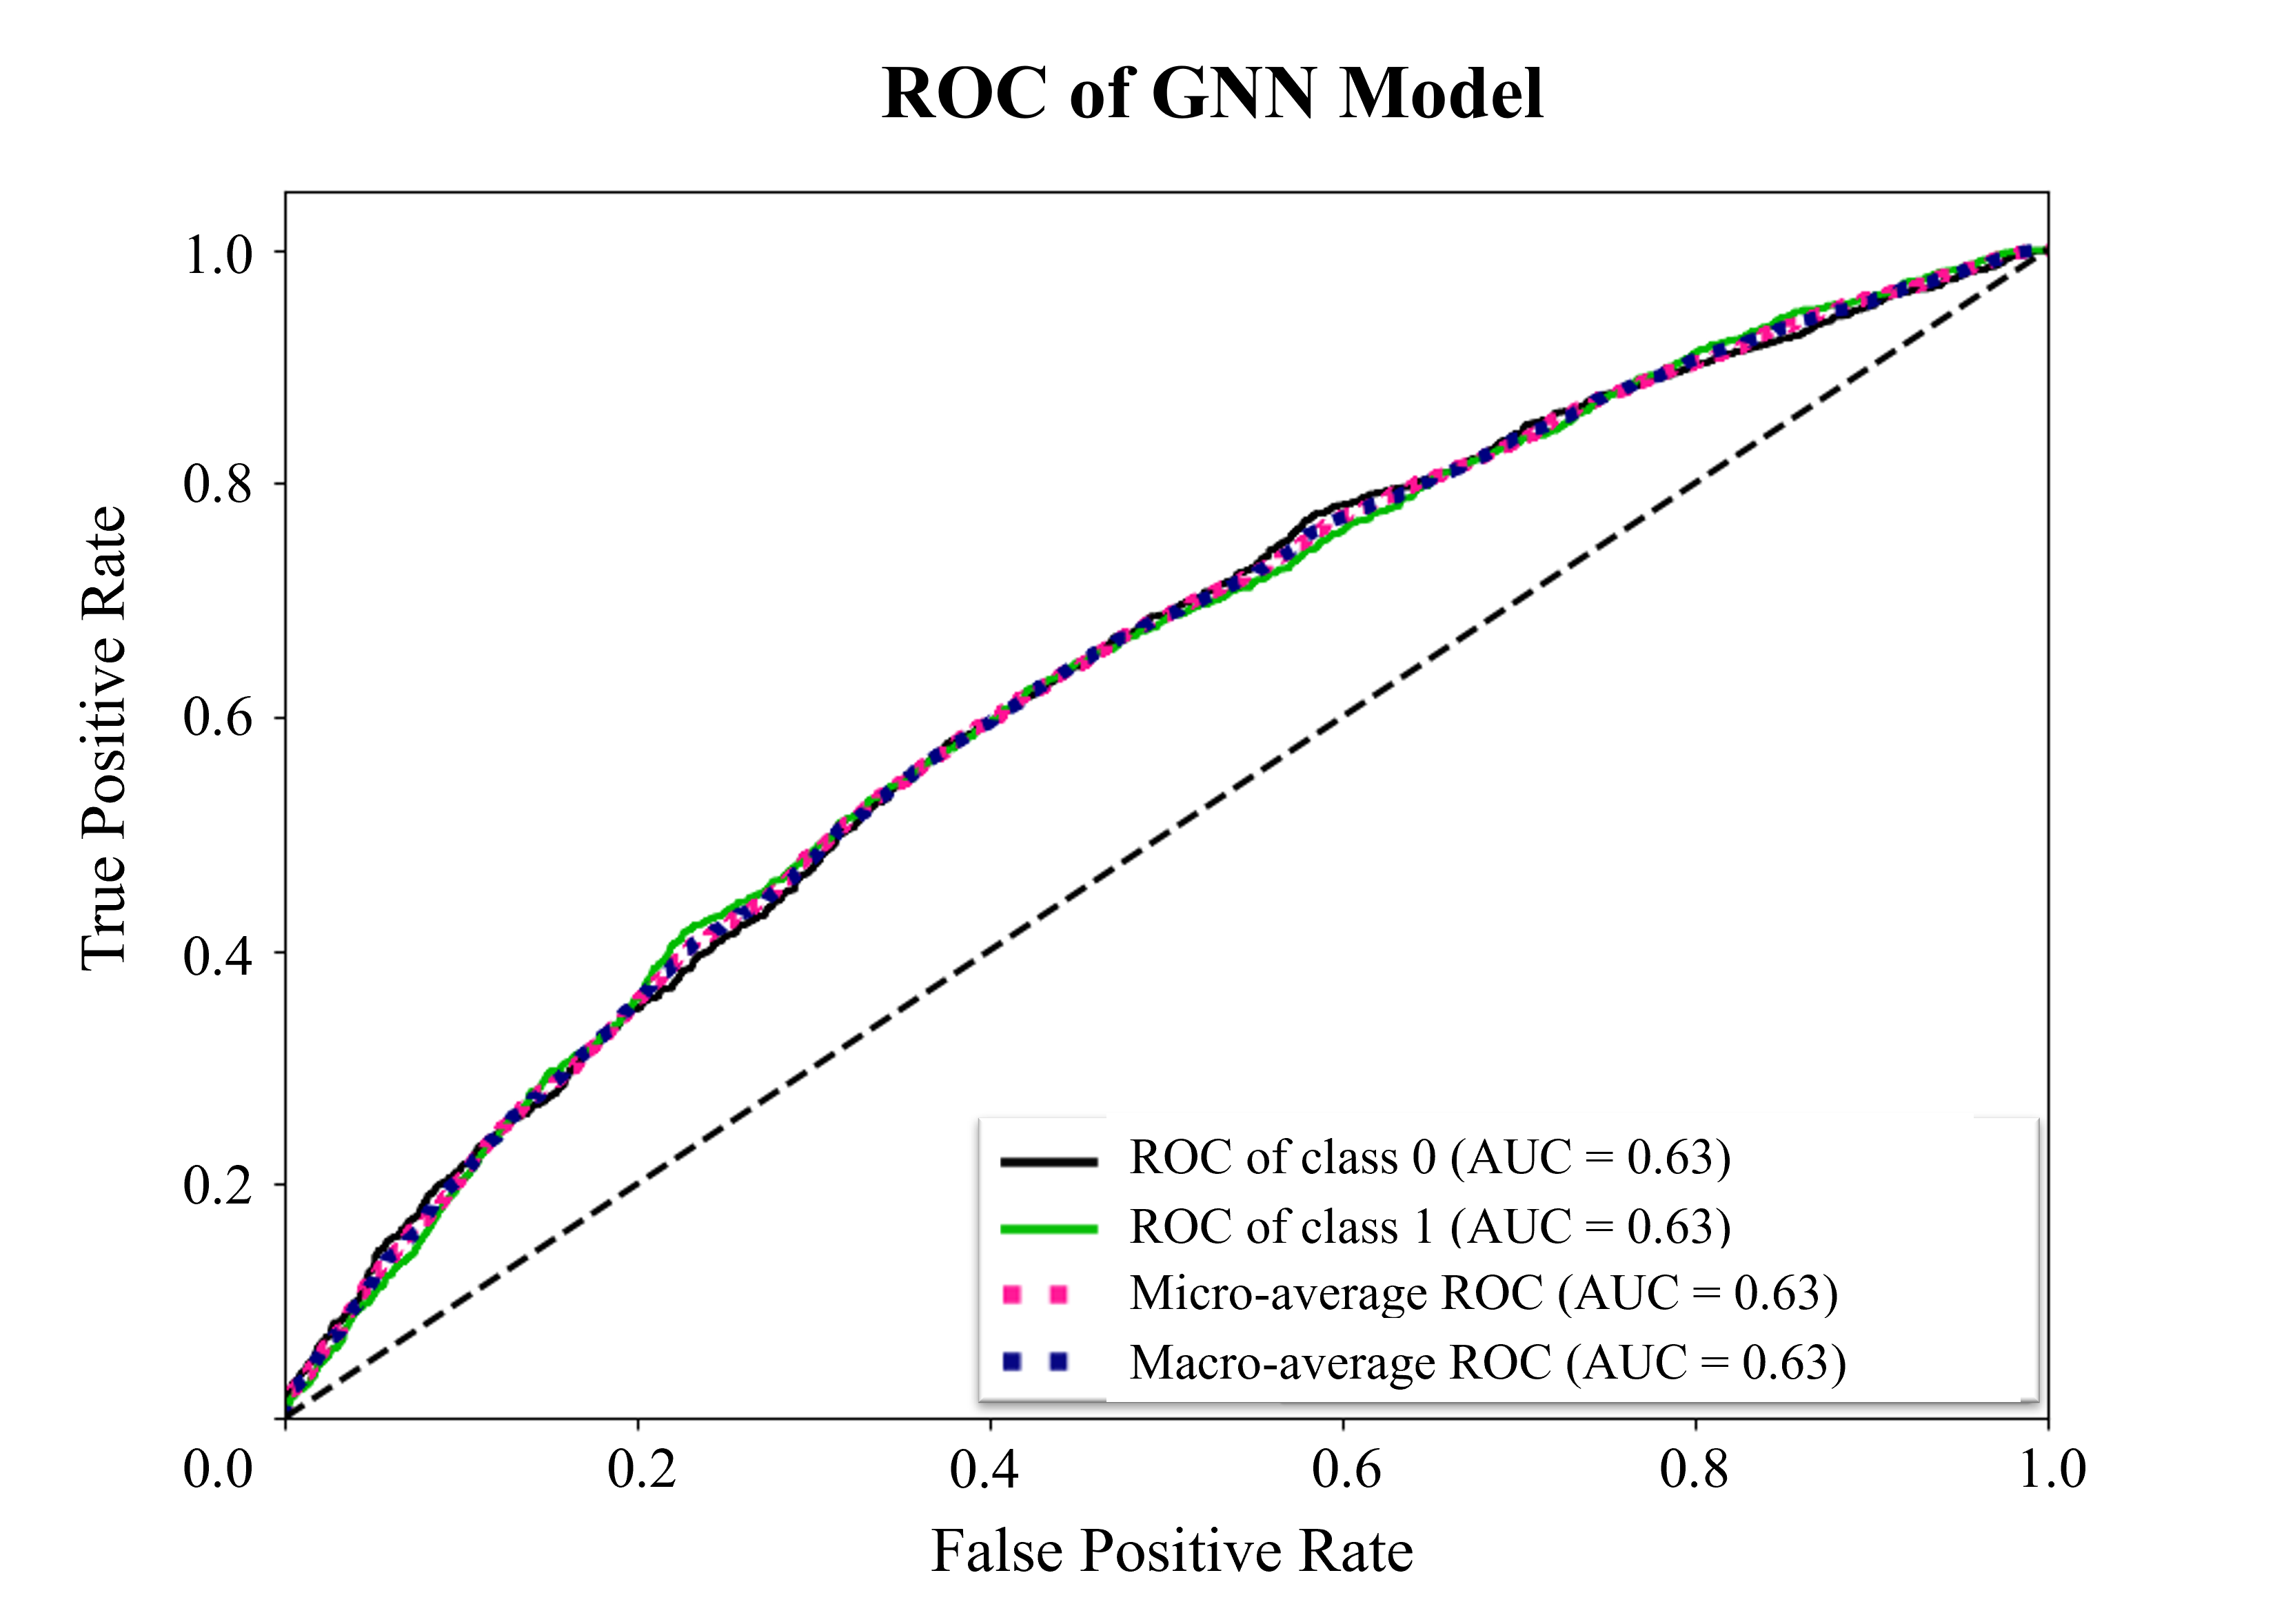
\includegraphics[width=7.5cm]{figures/Chapter4/GNN/GNNROC.png}
}
\quad
\subfigure[PRS模型ROC曲线]{
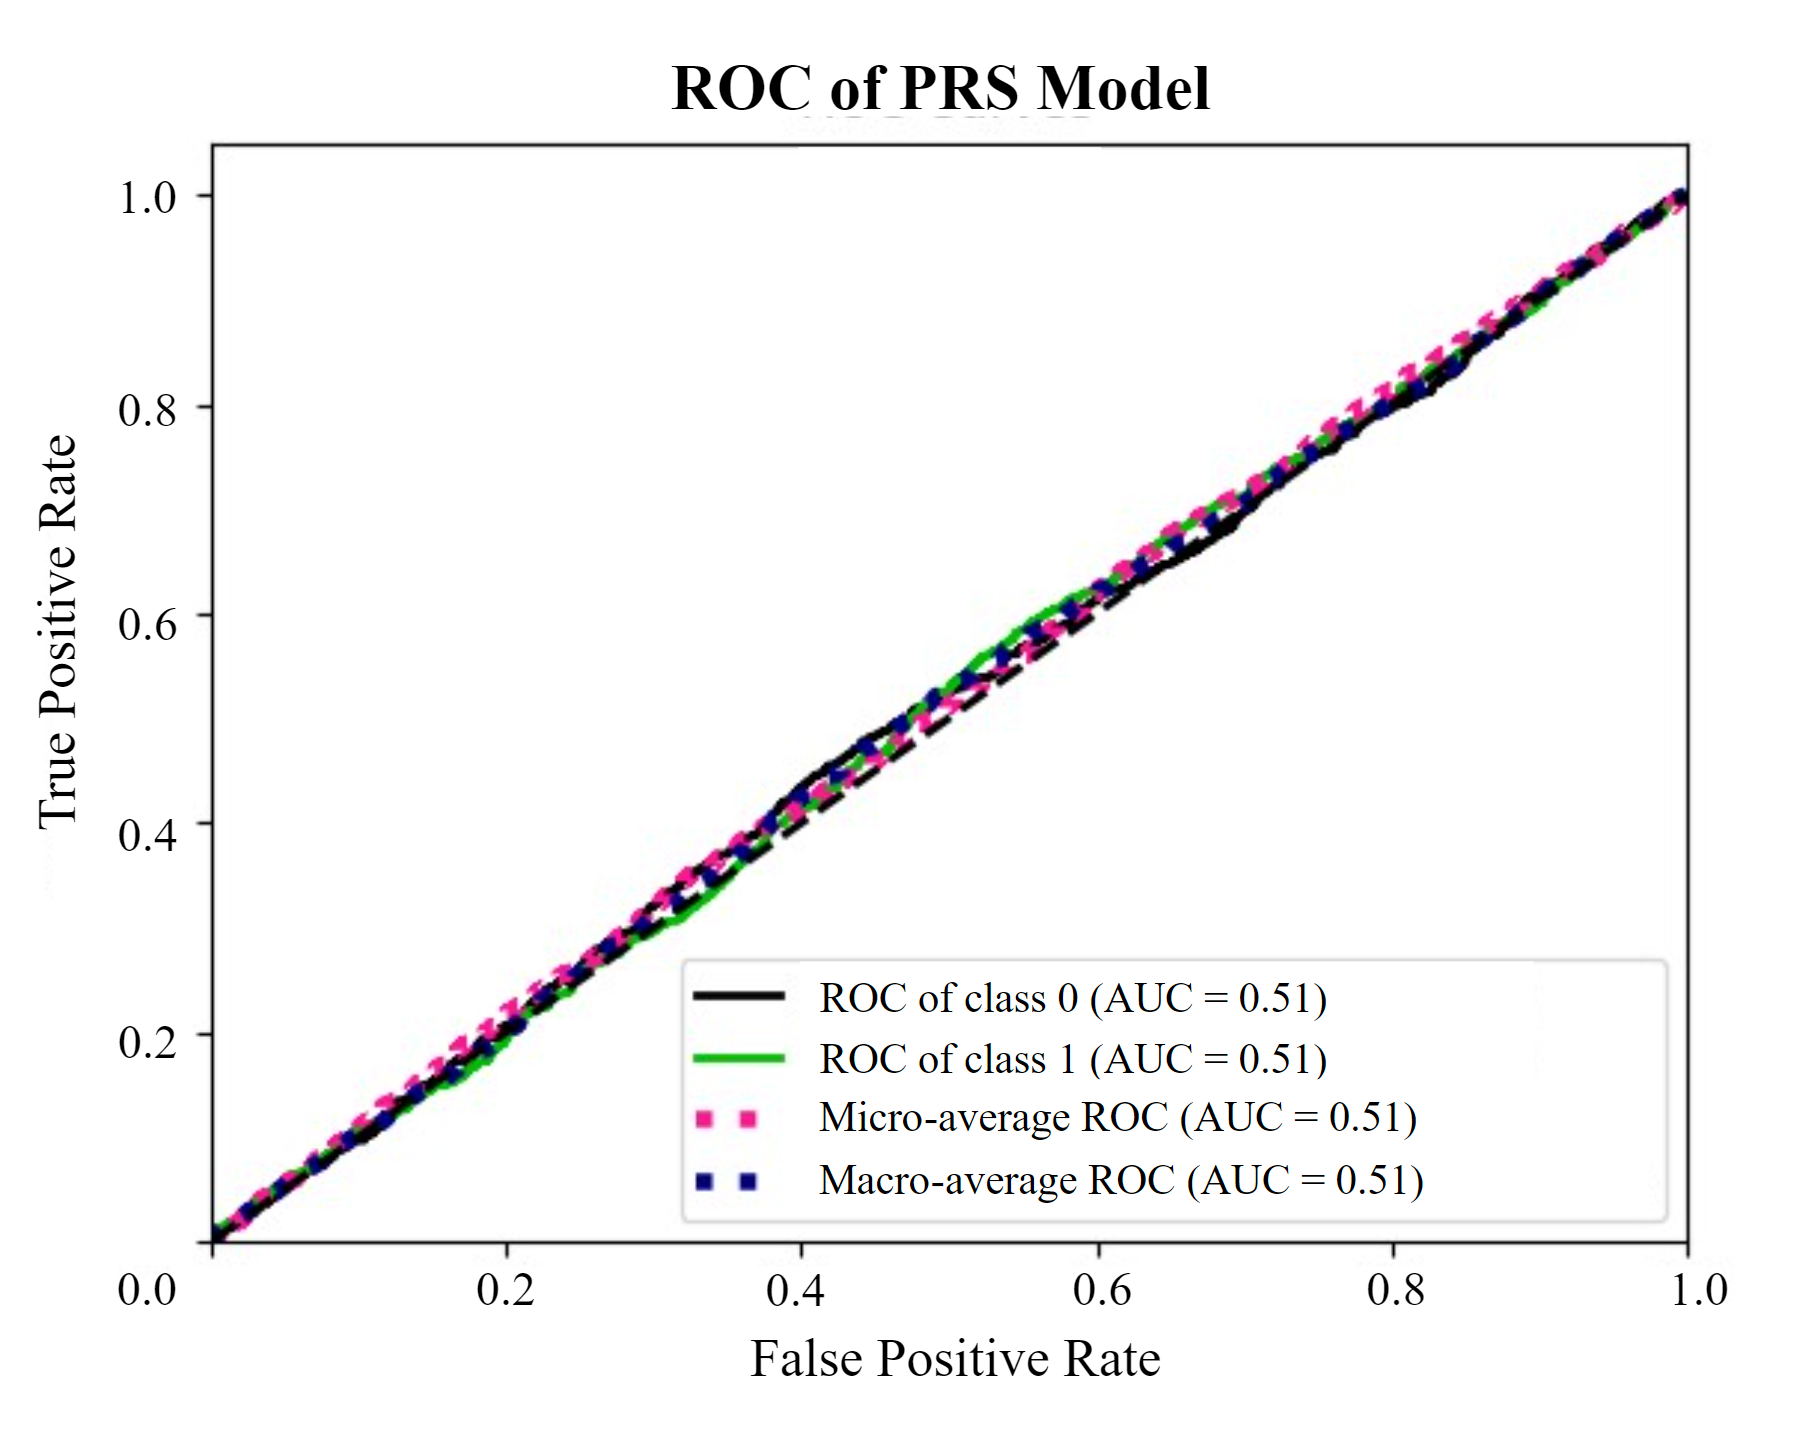
\includegraphics[width=7cm]{figures/Chapter4/GNN/PRSROC.png}
}
\quad
\subfigure[图神经网络模型Lift曲线]{
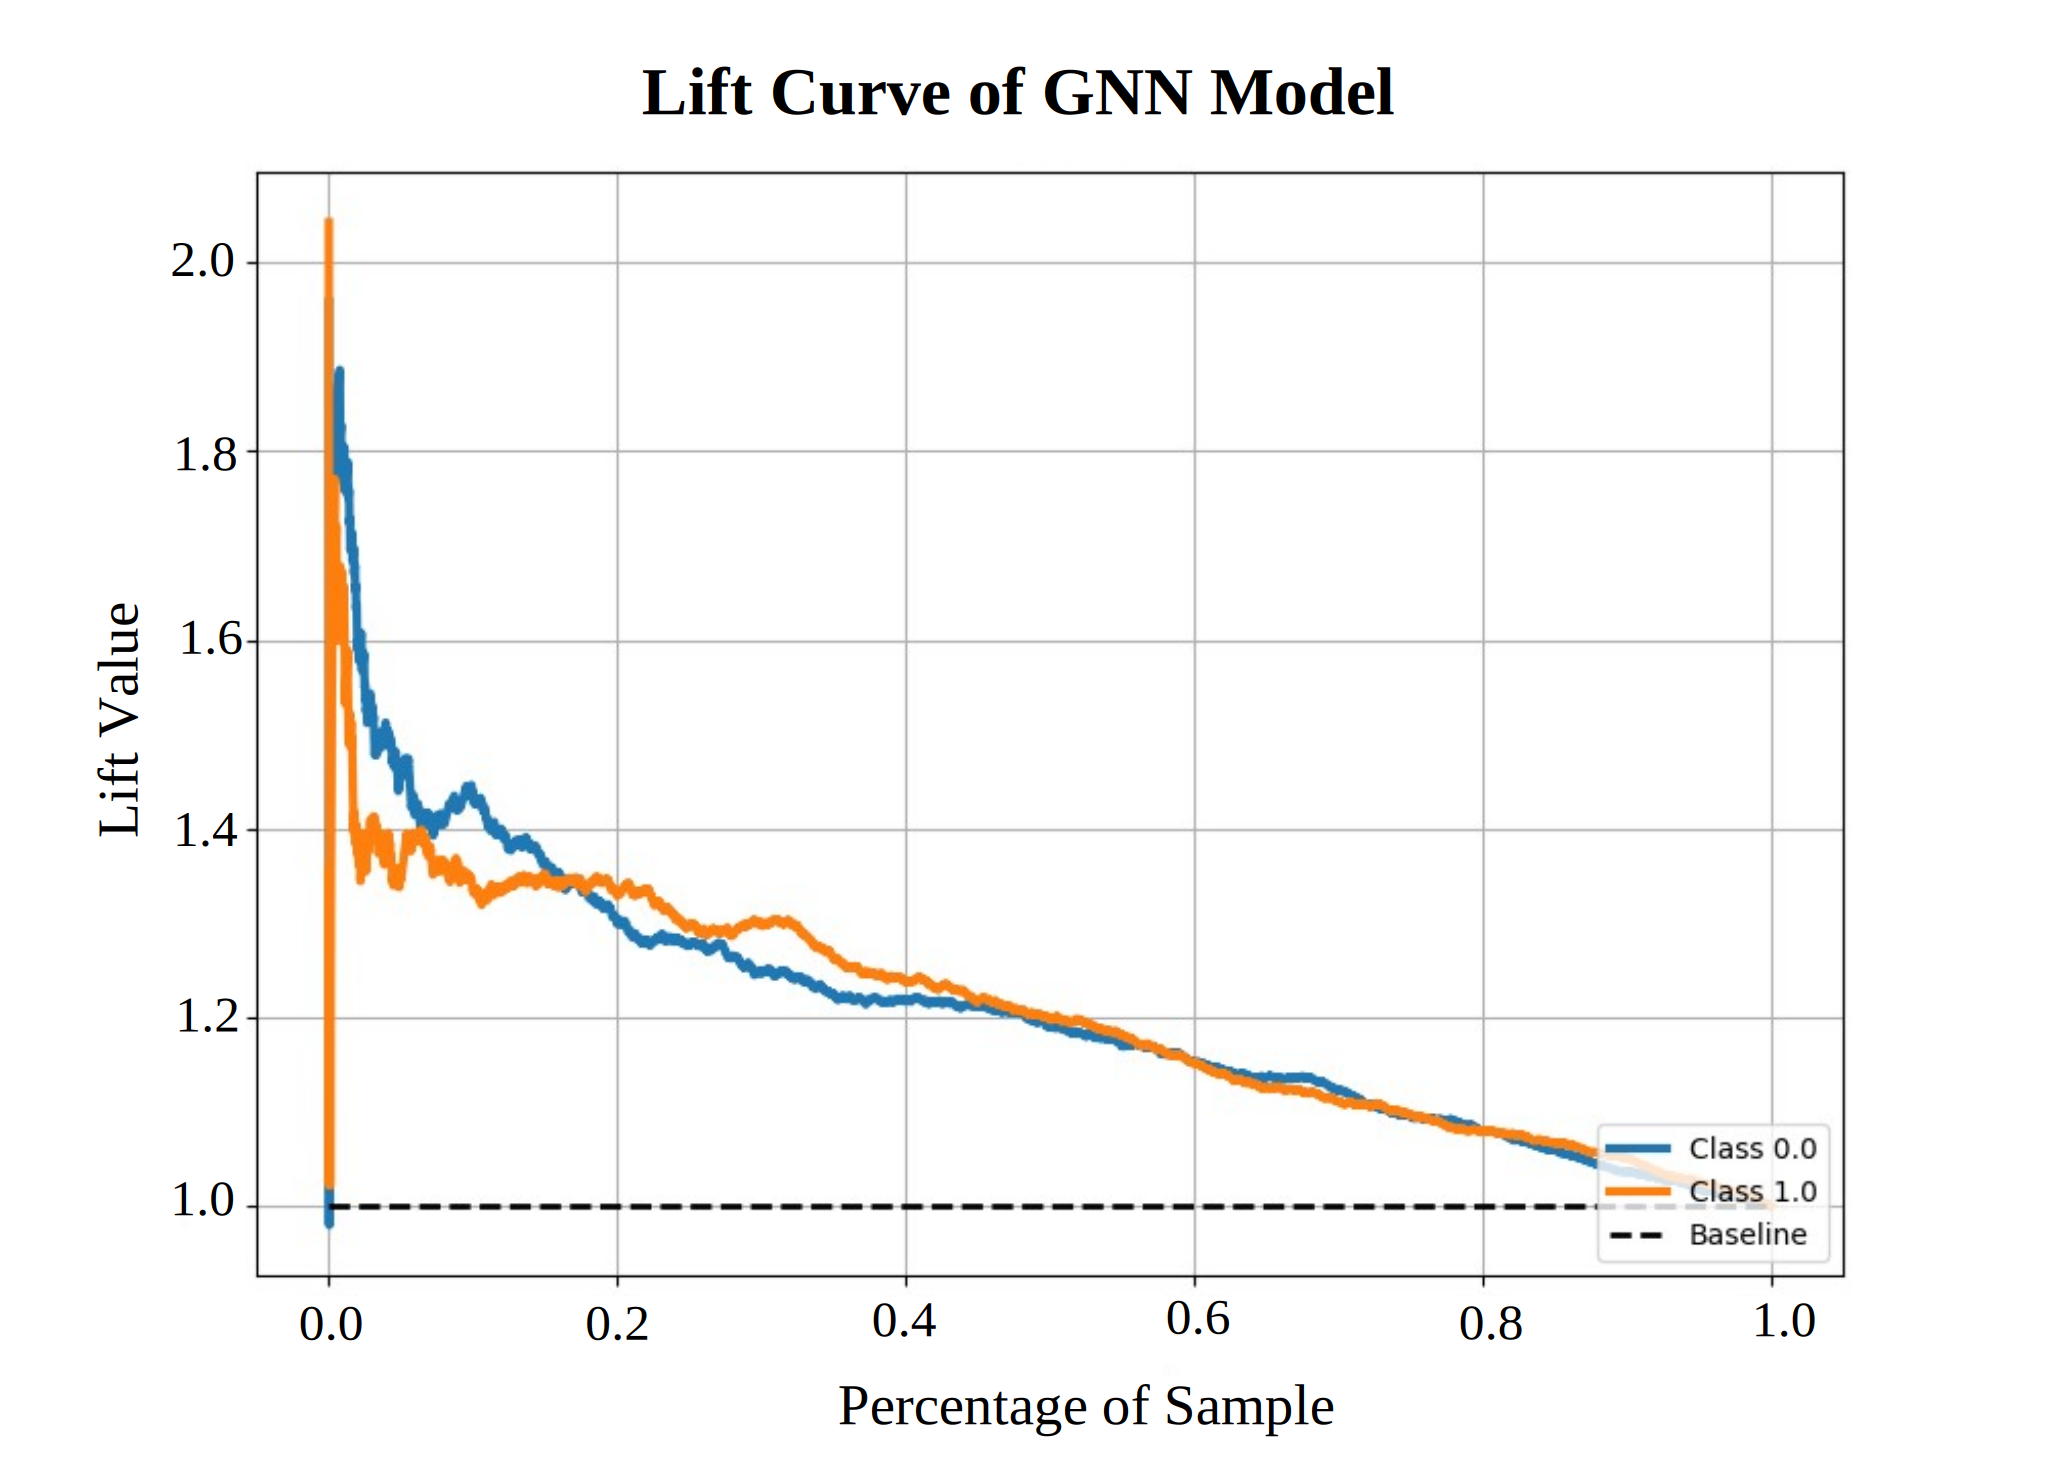
\includegraphics[width=9cm]{figures/Chapter4/GNN/GNNlift.png}
}
\quad
\subfigure[图神经网络模型Precision-Recall曲线]{
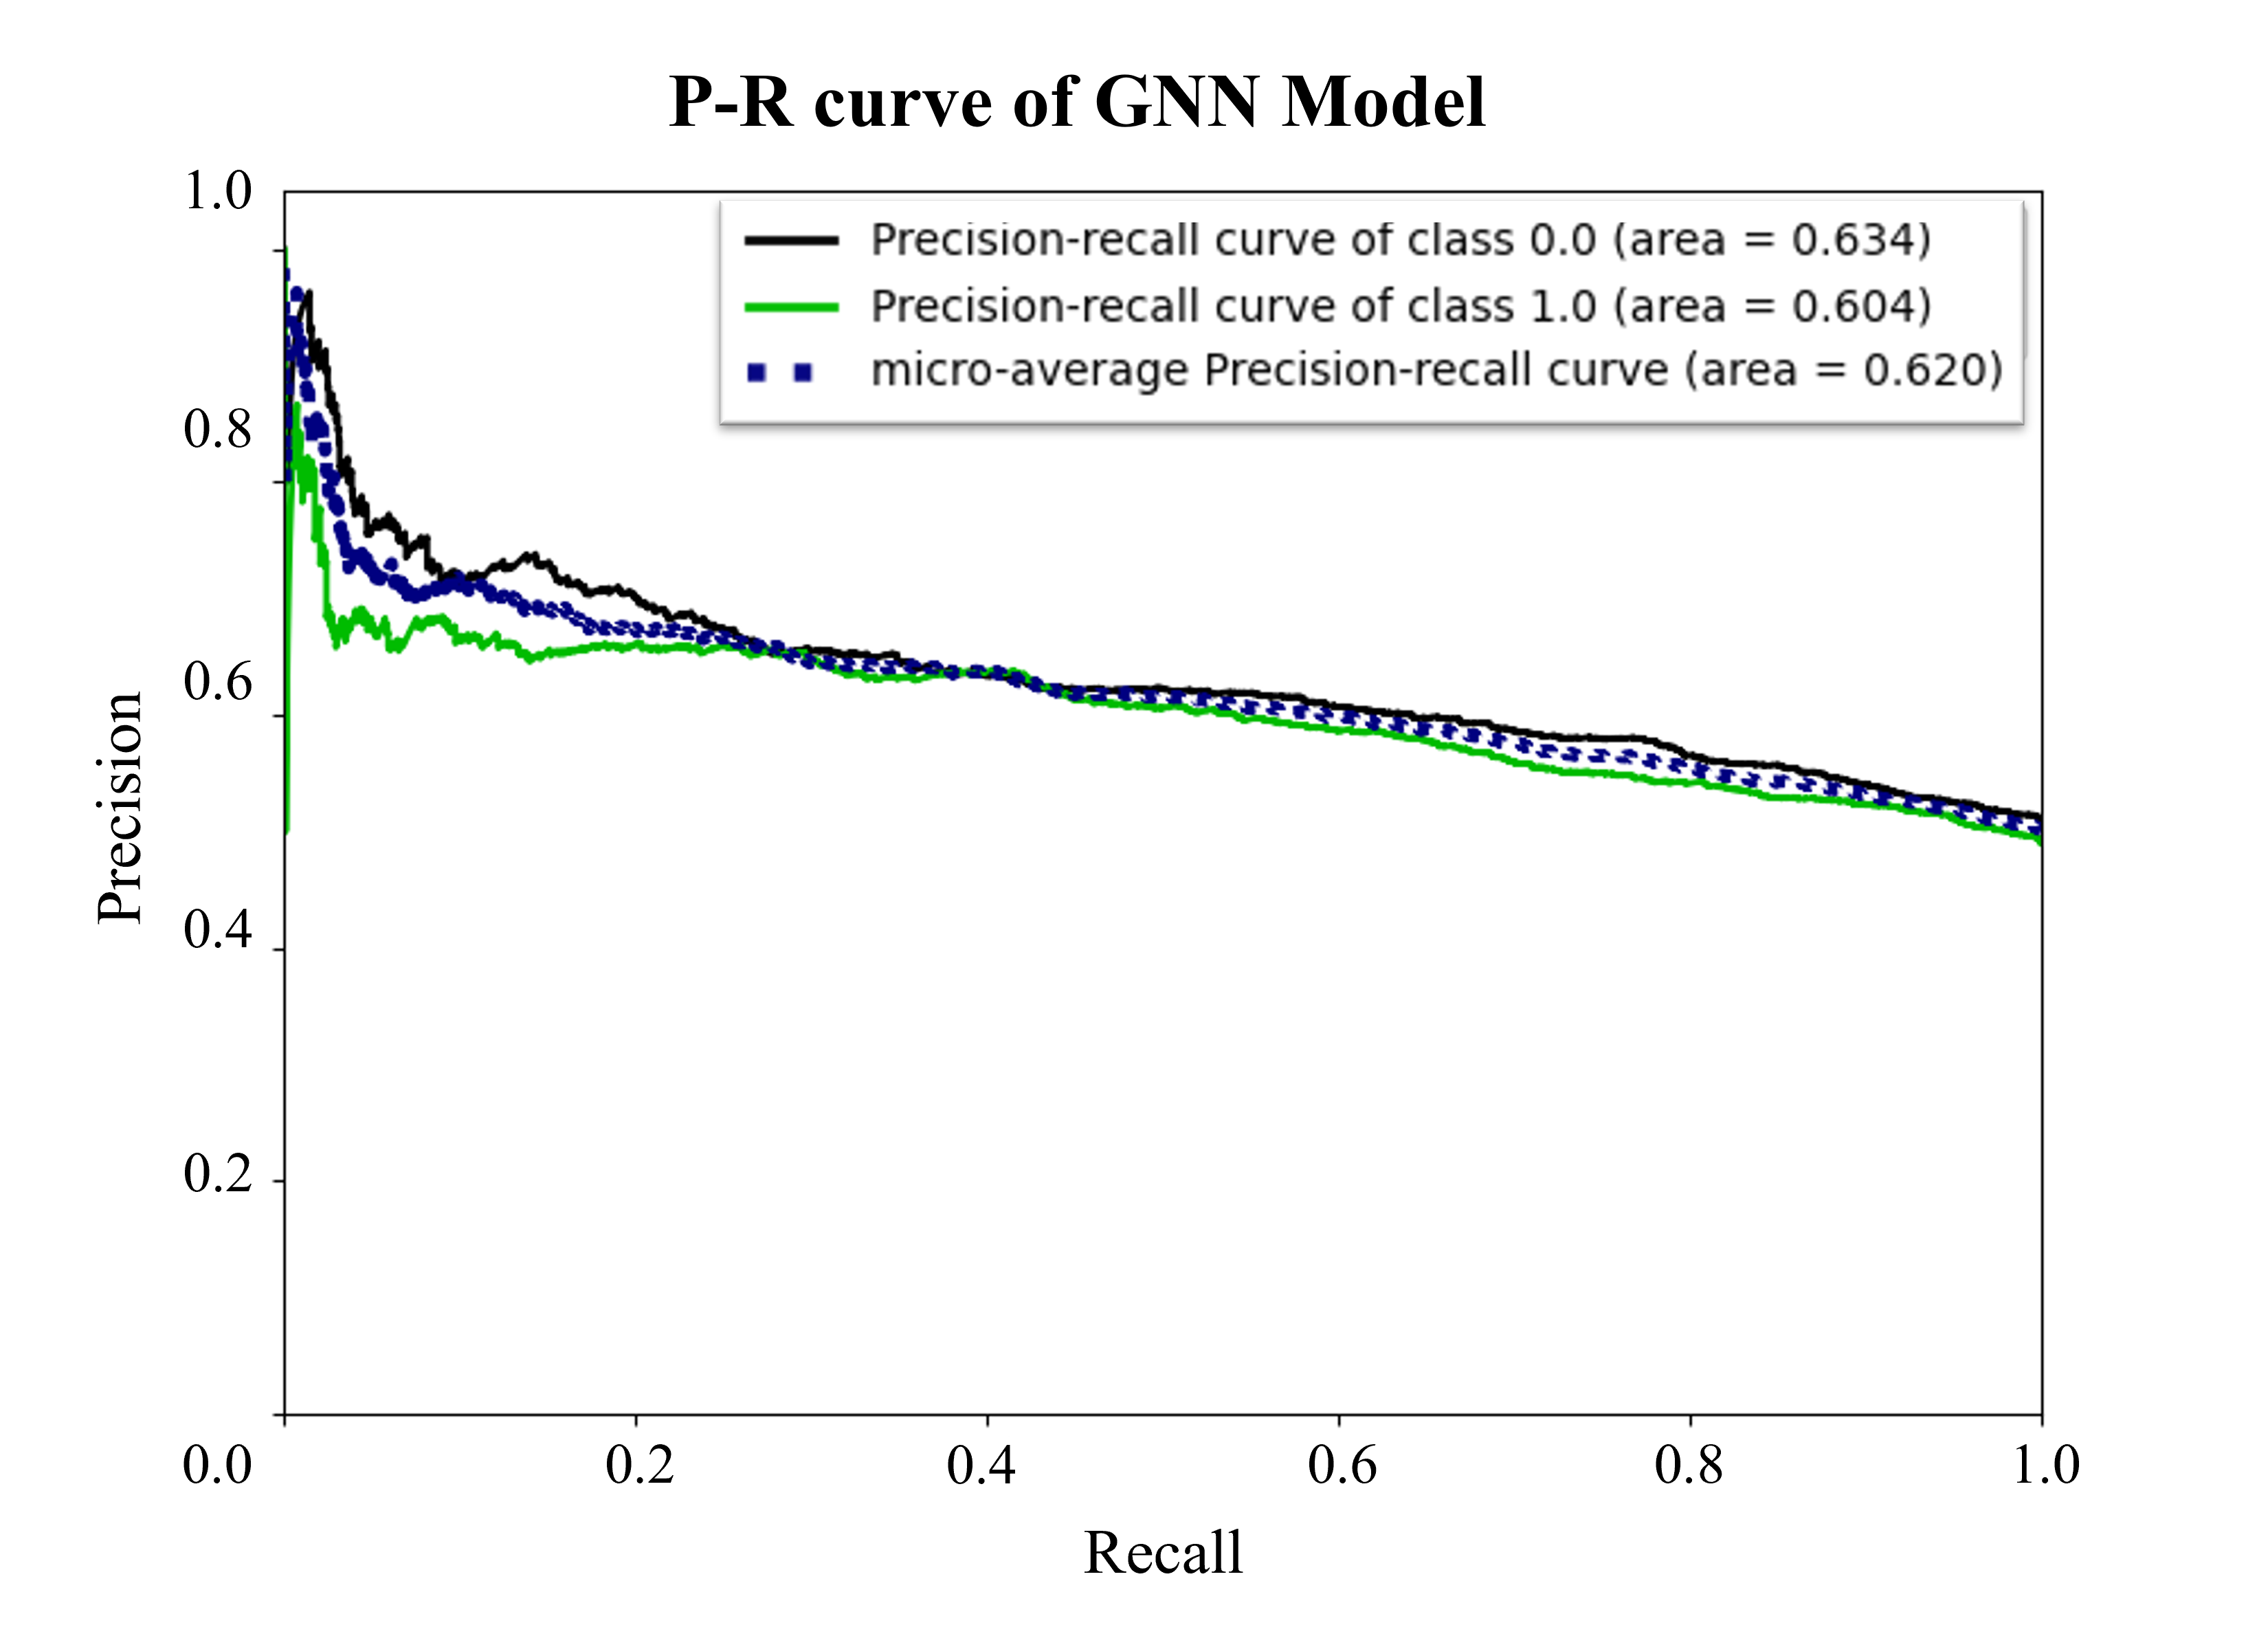
\includegraphics[width=9cm]{figures/Chapter4/GNN/GNNPR.png}
}
\caption{图神经网络模型性能曲线}
\end{figure}



可以看出,本文建立的图神经网络较PRS模型及传统机器学习模型性能有了明显改善。证明了图神经网络在处理图数据时的优秀效果。
\subsection{表型融合}
为进一步增强模型性能,本文引入同骨关节炎密切相关的表型参与风险预测,其给出如下结果。
\begin{table}[!h]
	\renewcommand{\arraystretch}{1.2}
	\centering\wuhao
	\caption{融合表型信息对模型性能的影响} \label{ICD_exclude} \vspace{2mm}
	\begin{tabularx}{\textwidth} { 
   >{\centering\arraybackslash}X 
   >{\centering\arraybackslash}X
   >{\centering\arraybackslash}X
   >{\centering\arraybackslash}X}
	\toprule[1.5pt]
	指标 & 融合表型 & 单纯图神经网络 & PRS模型 \\
	\midrule[1pt]
auc & 0.74 & 0.60 & 0.51 \\
f1 & 0.66 & 0.57 & 0.45 \\
accuracy & 0.67 & 0.58 & 0.52 \\
precision & 0.66 & 0.57 & 0.50 \\
recall & 0.69 & 0.58 & 0.41 \\
	\bottomrule[1.5pt]
	\end{tabularx}
\end{table}
\begin{figure}[htbp]
\centering

\subfigure[融合表型模型ROC曲线]{
\includegraphics[width=7cm]{figures/Chapter4/GNN/PhenoROC.png}
}
\quad
\subfigure[单纯图神经网络模型ROC曲线]{
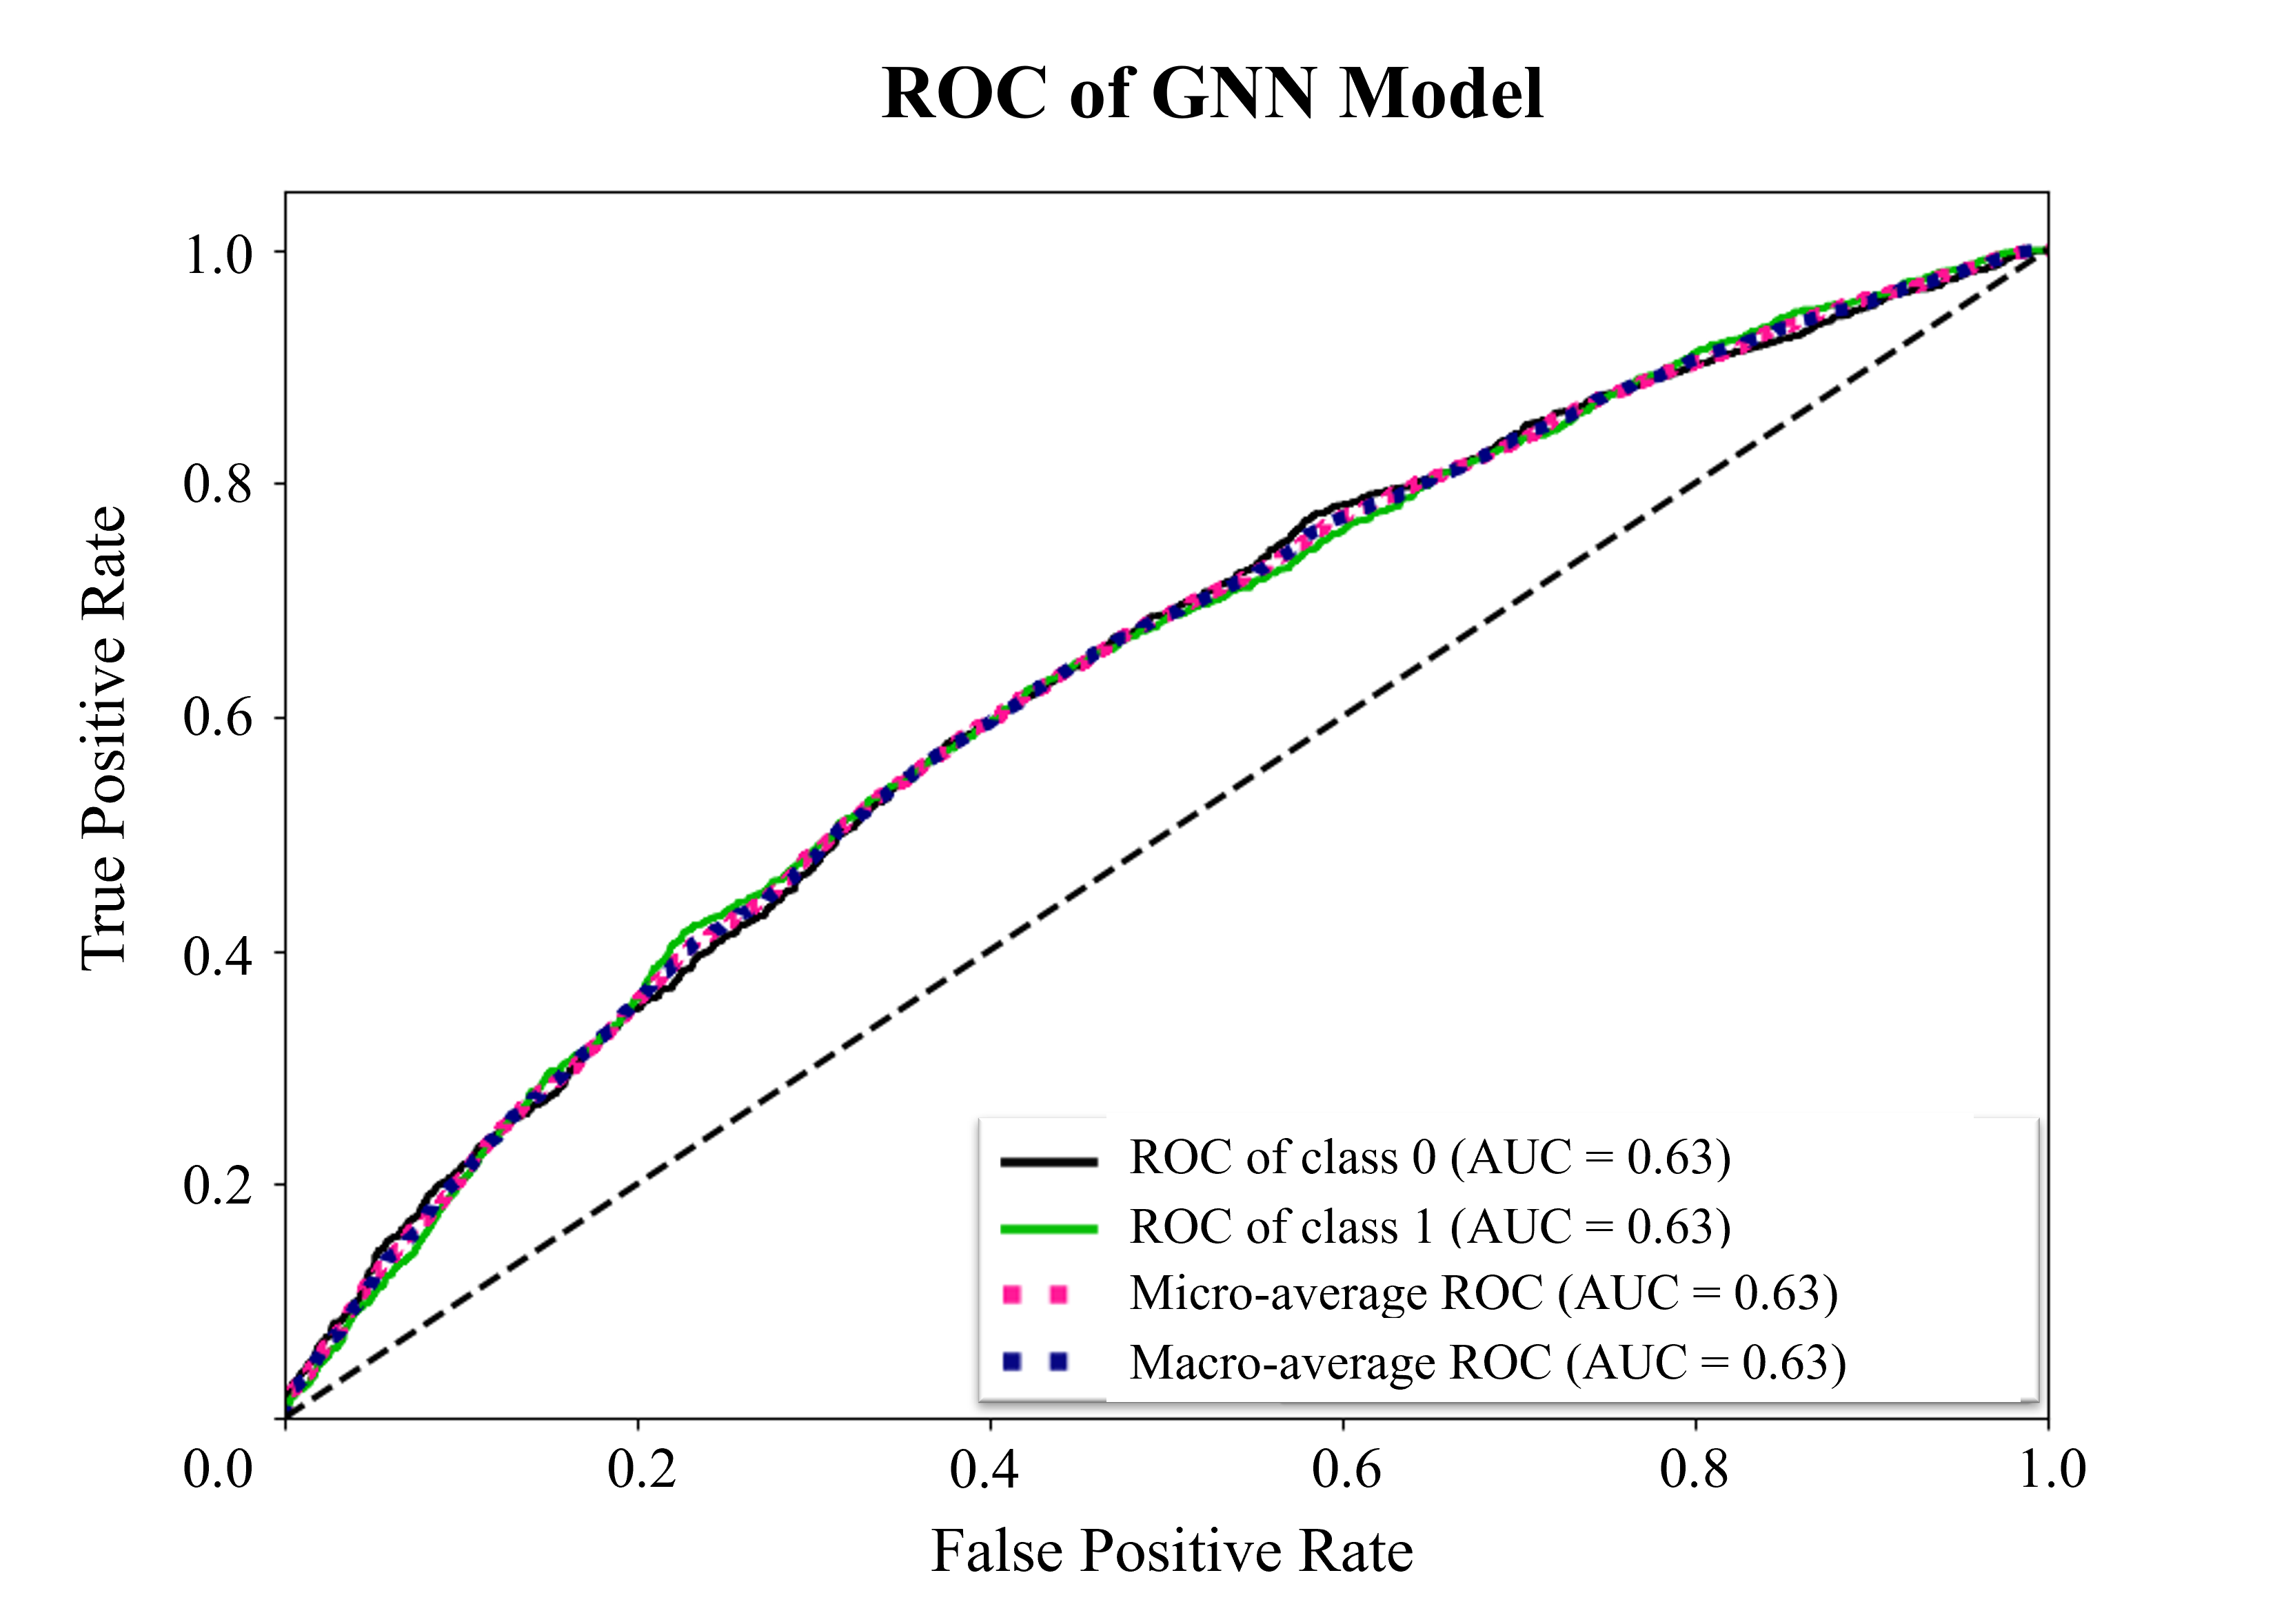
\includegraphics[width=7cm]{figures/Chapter4/GNN/GNNROC.png}
}
\quad
\subfigure[融合表型模型KS曲线]{
\includegraphics[width=7cm]{figures/Chapter4/GNN/PhenoKS.png}
}
\quad
\subfigure[单纯图神经网络模型KS曲线]{
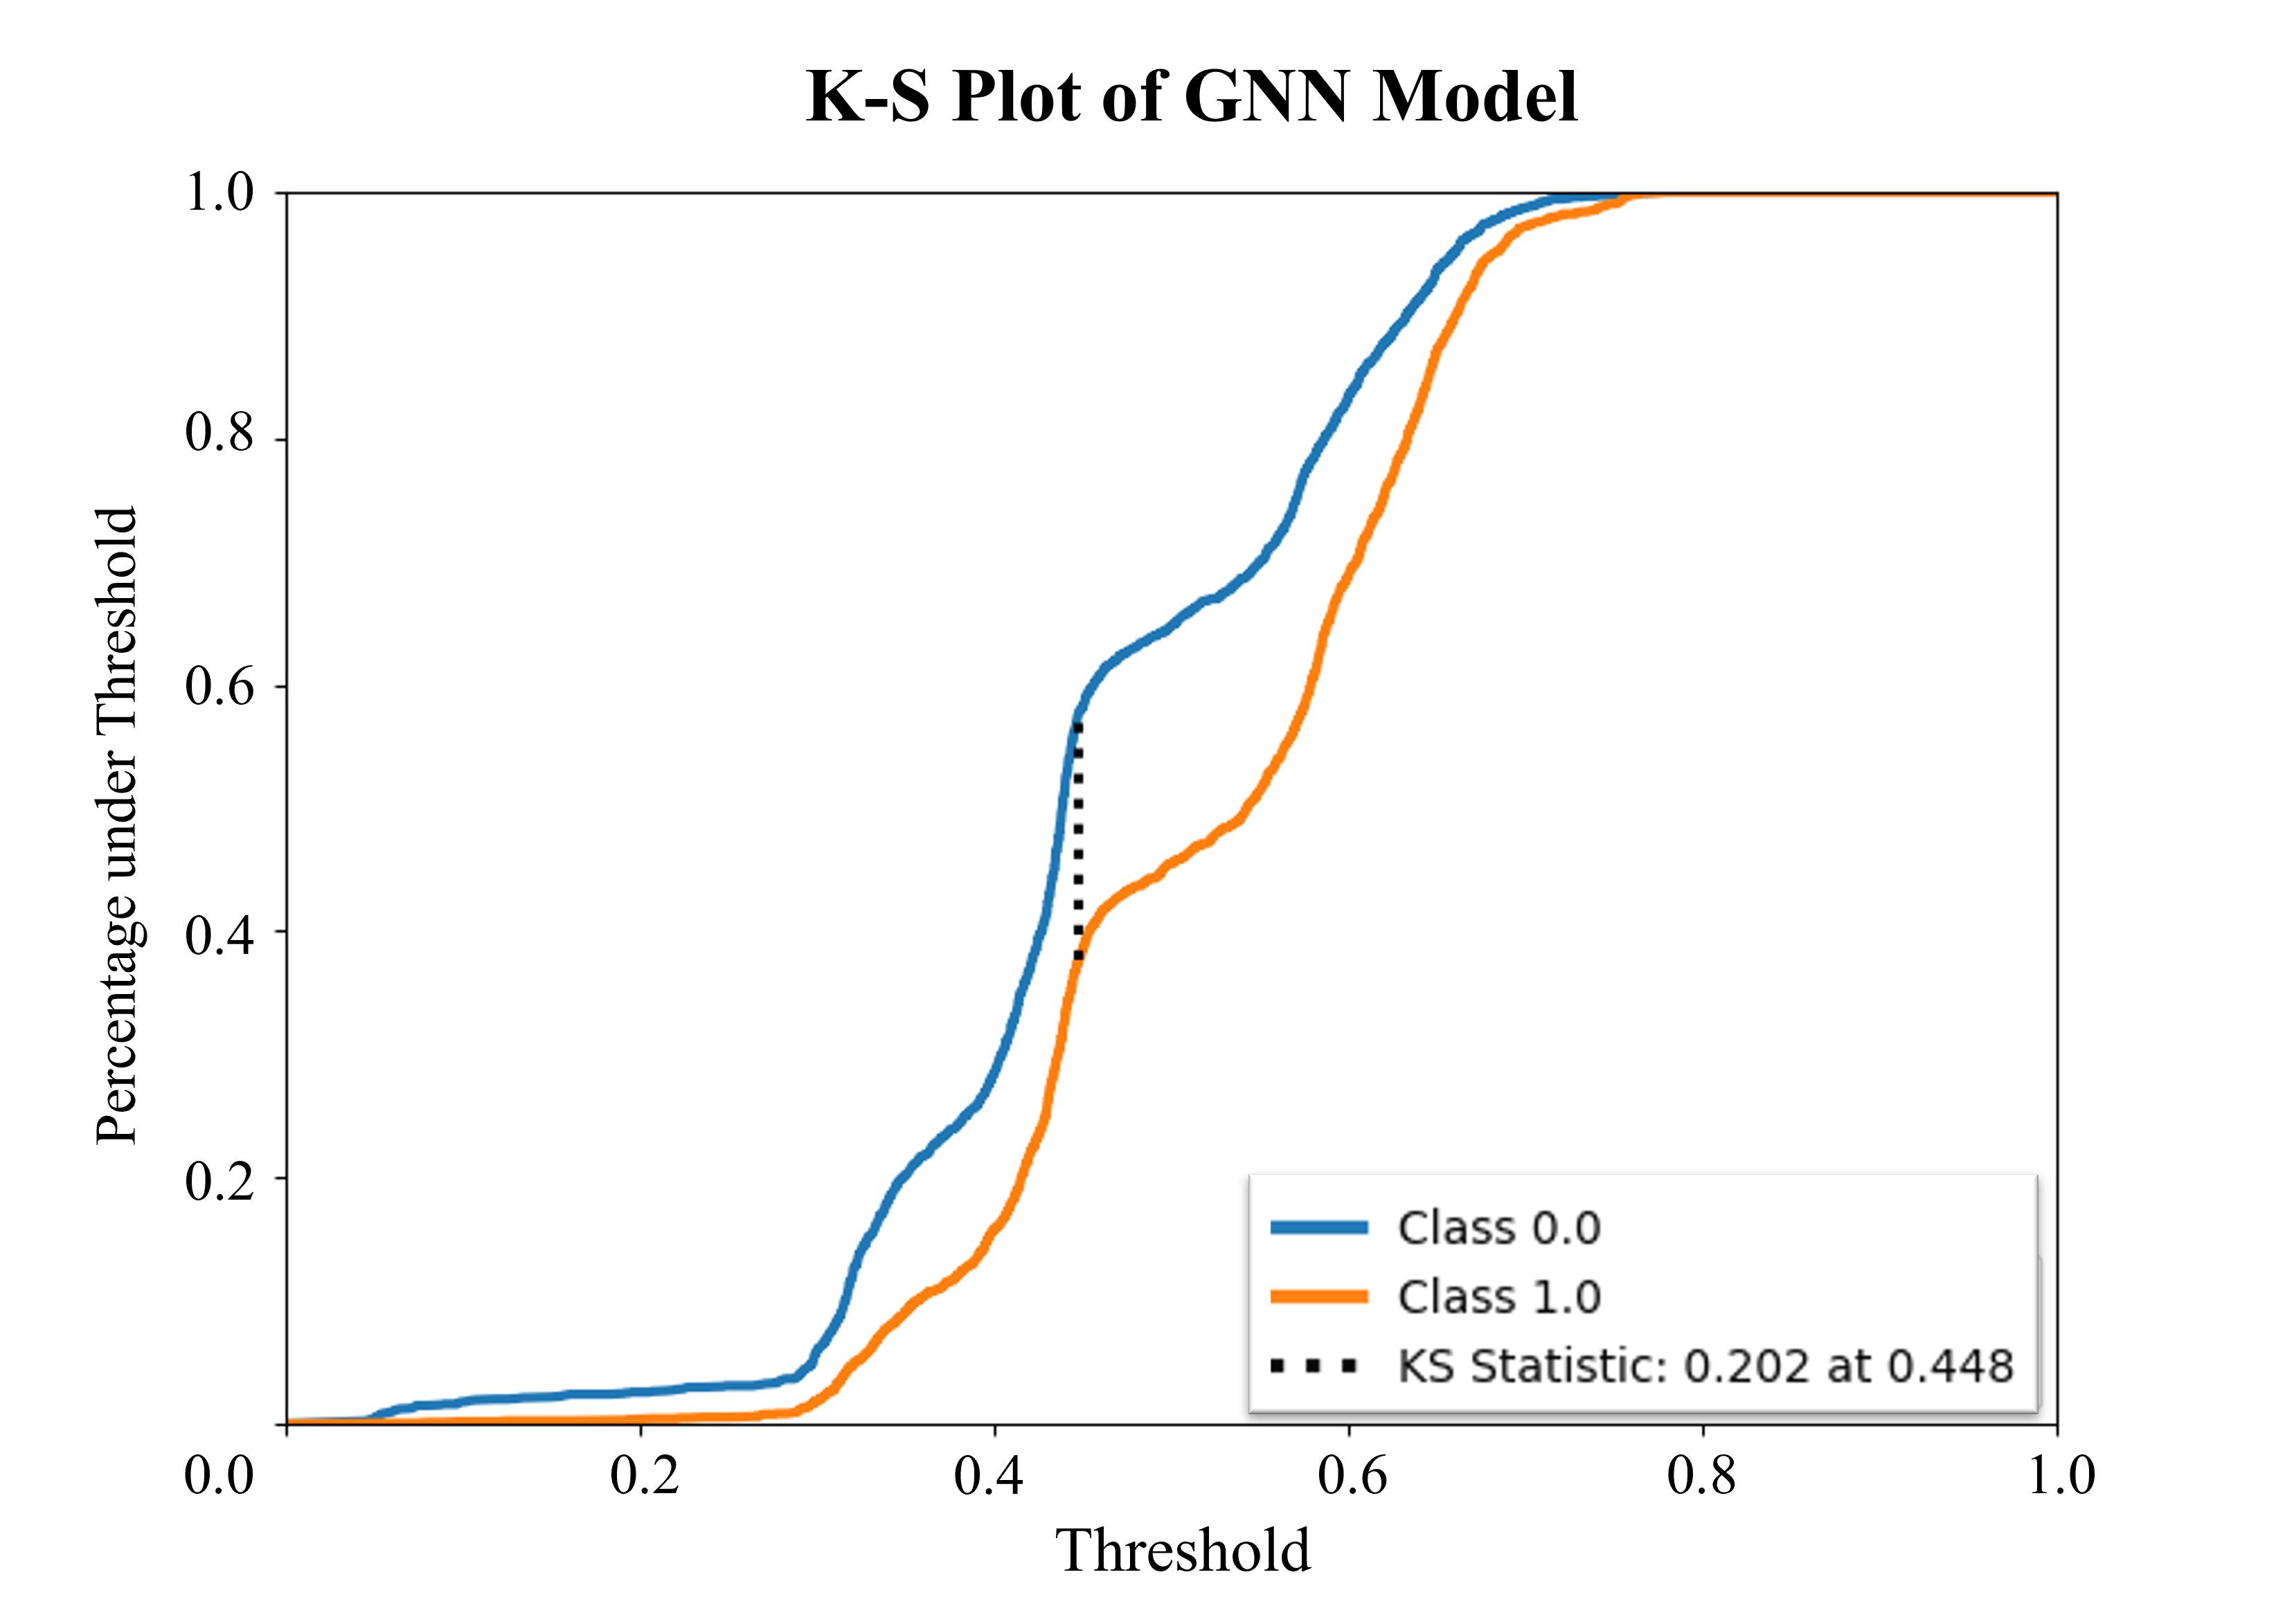
\includegraphics[width=7cm]{figures/Chapter4/GNN/GNNKS.png}
}
\quad
\subfigure[融合表型模型Lift曲线]{
\includegraphics[width=7cm]{figures/Chapter4/GNN/Phenolift.png}
}
\quad
\subfigure[单纯图神经网络模型Lift曲线]{
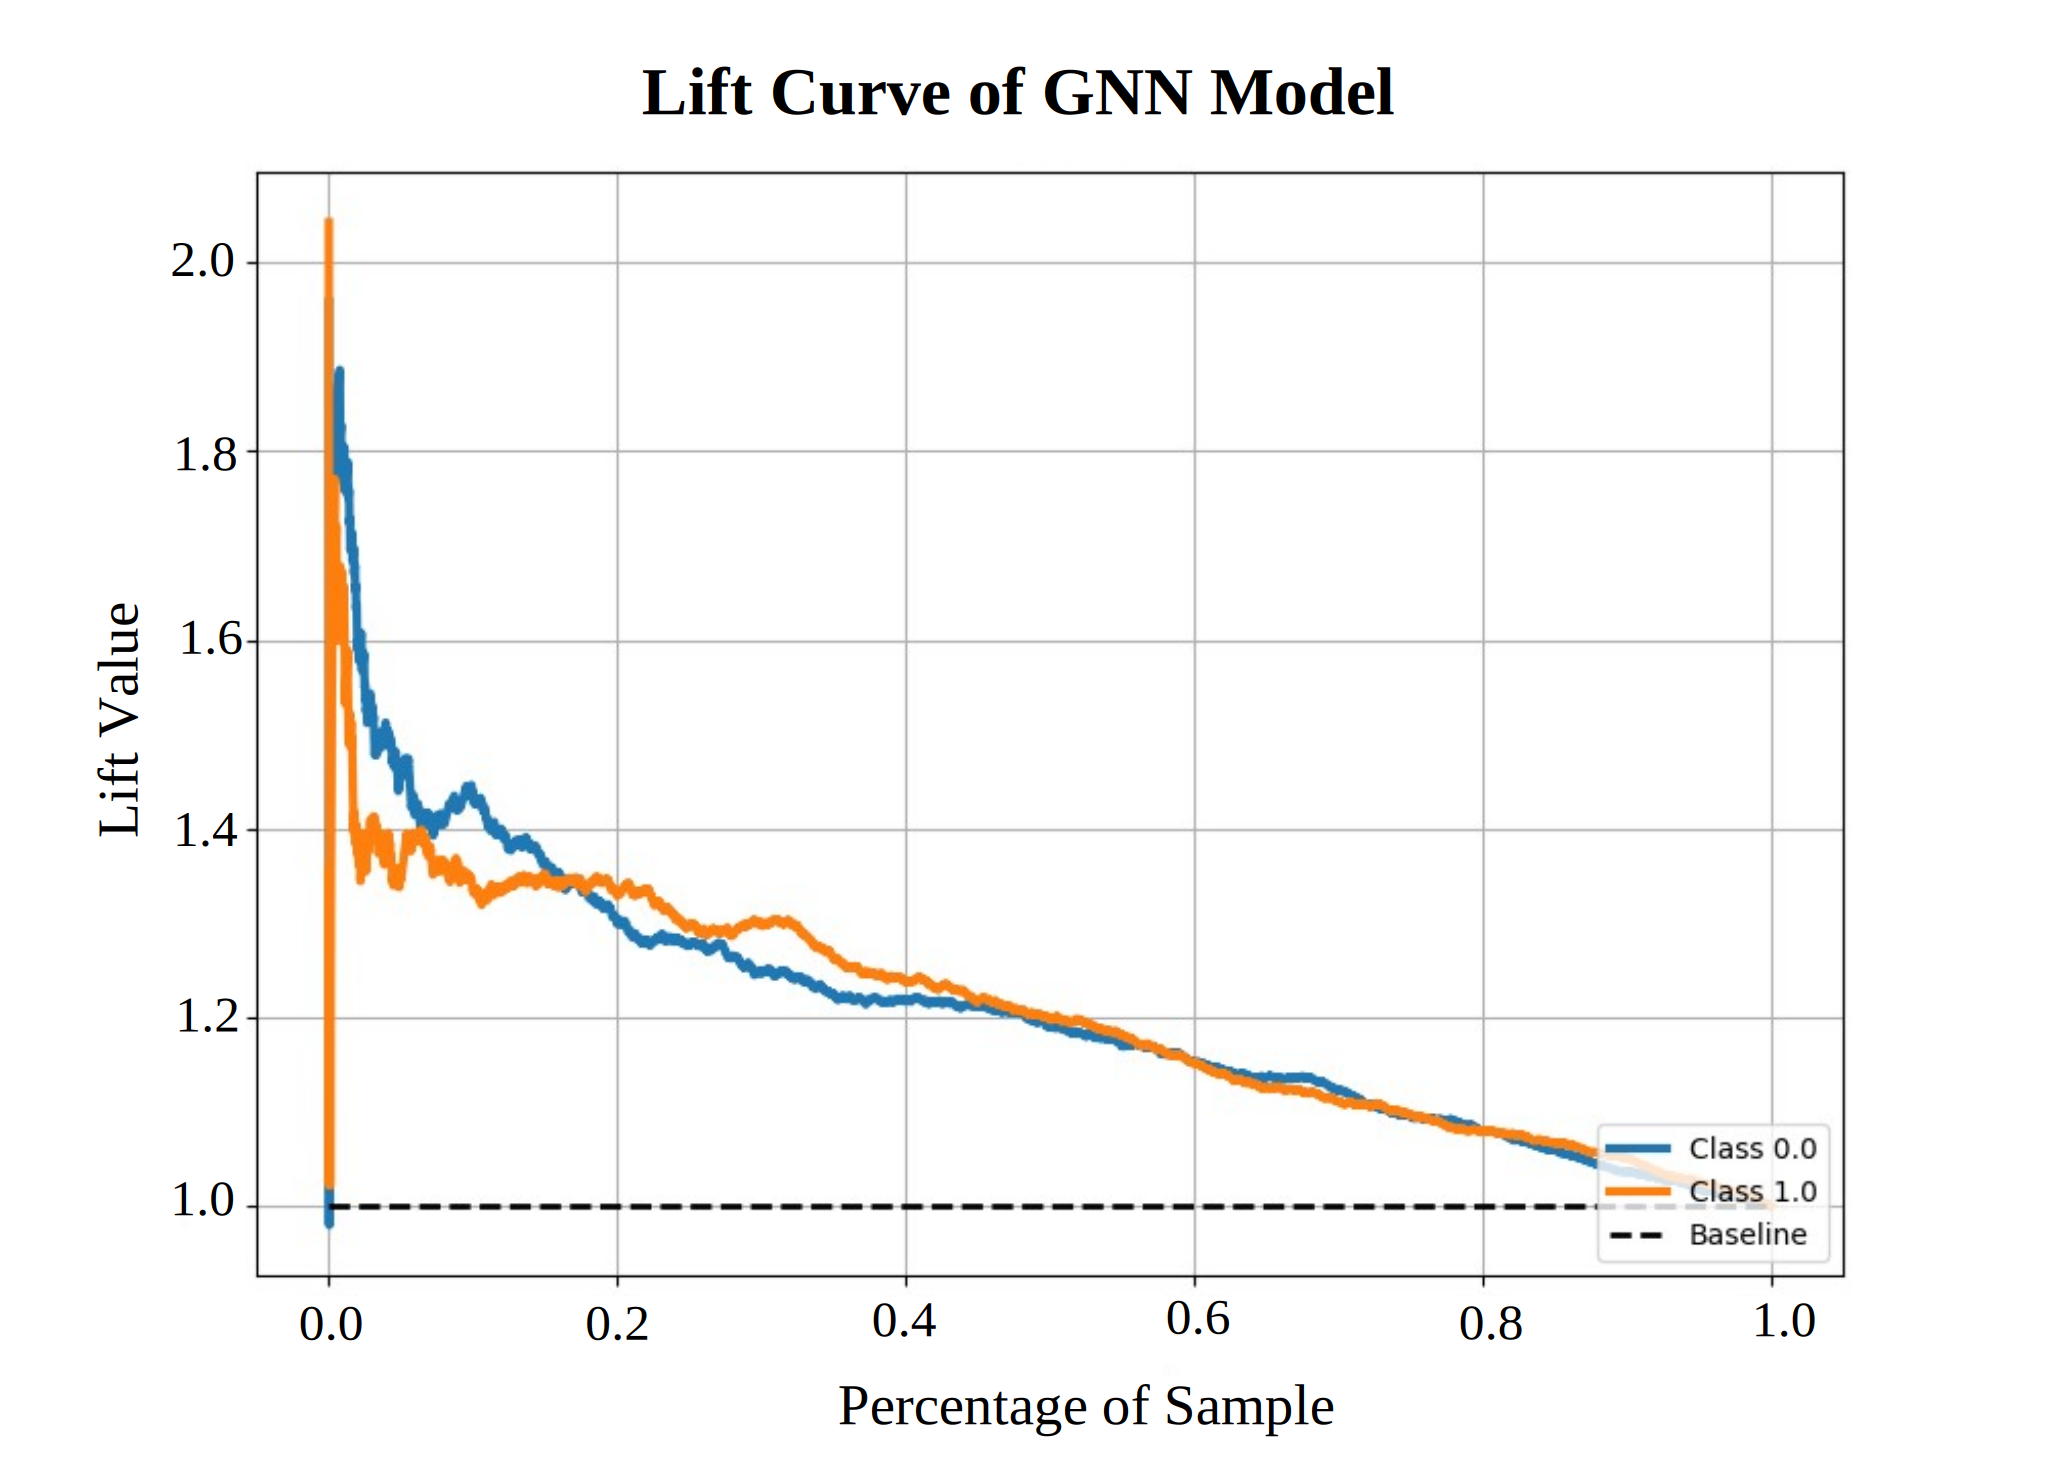
\includegraphics[width=7cm]{figures/Chapter4/GNN/GNNlift.png}
}
\quad
\subfigure[融合表型模型Precision-Recall曲线]{
\includegraphics[width=7cm]{figures/Chapter4/GNN/PhenoPR.png}
}
\quad
\subfigure[单纯图神经网络模型Precision-Recall曲线]{
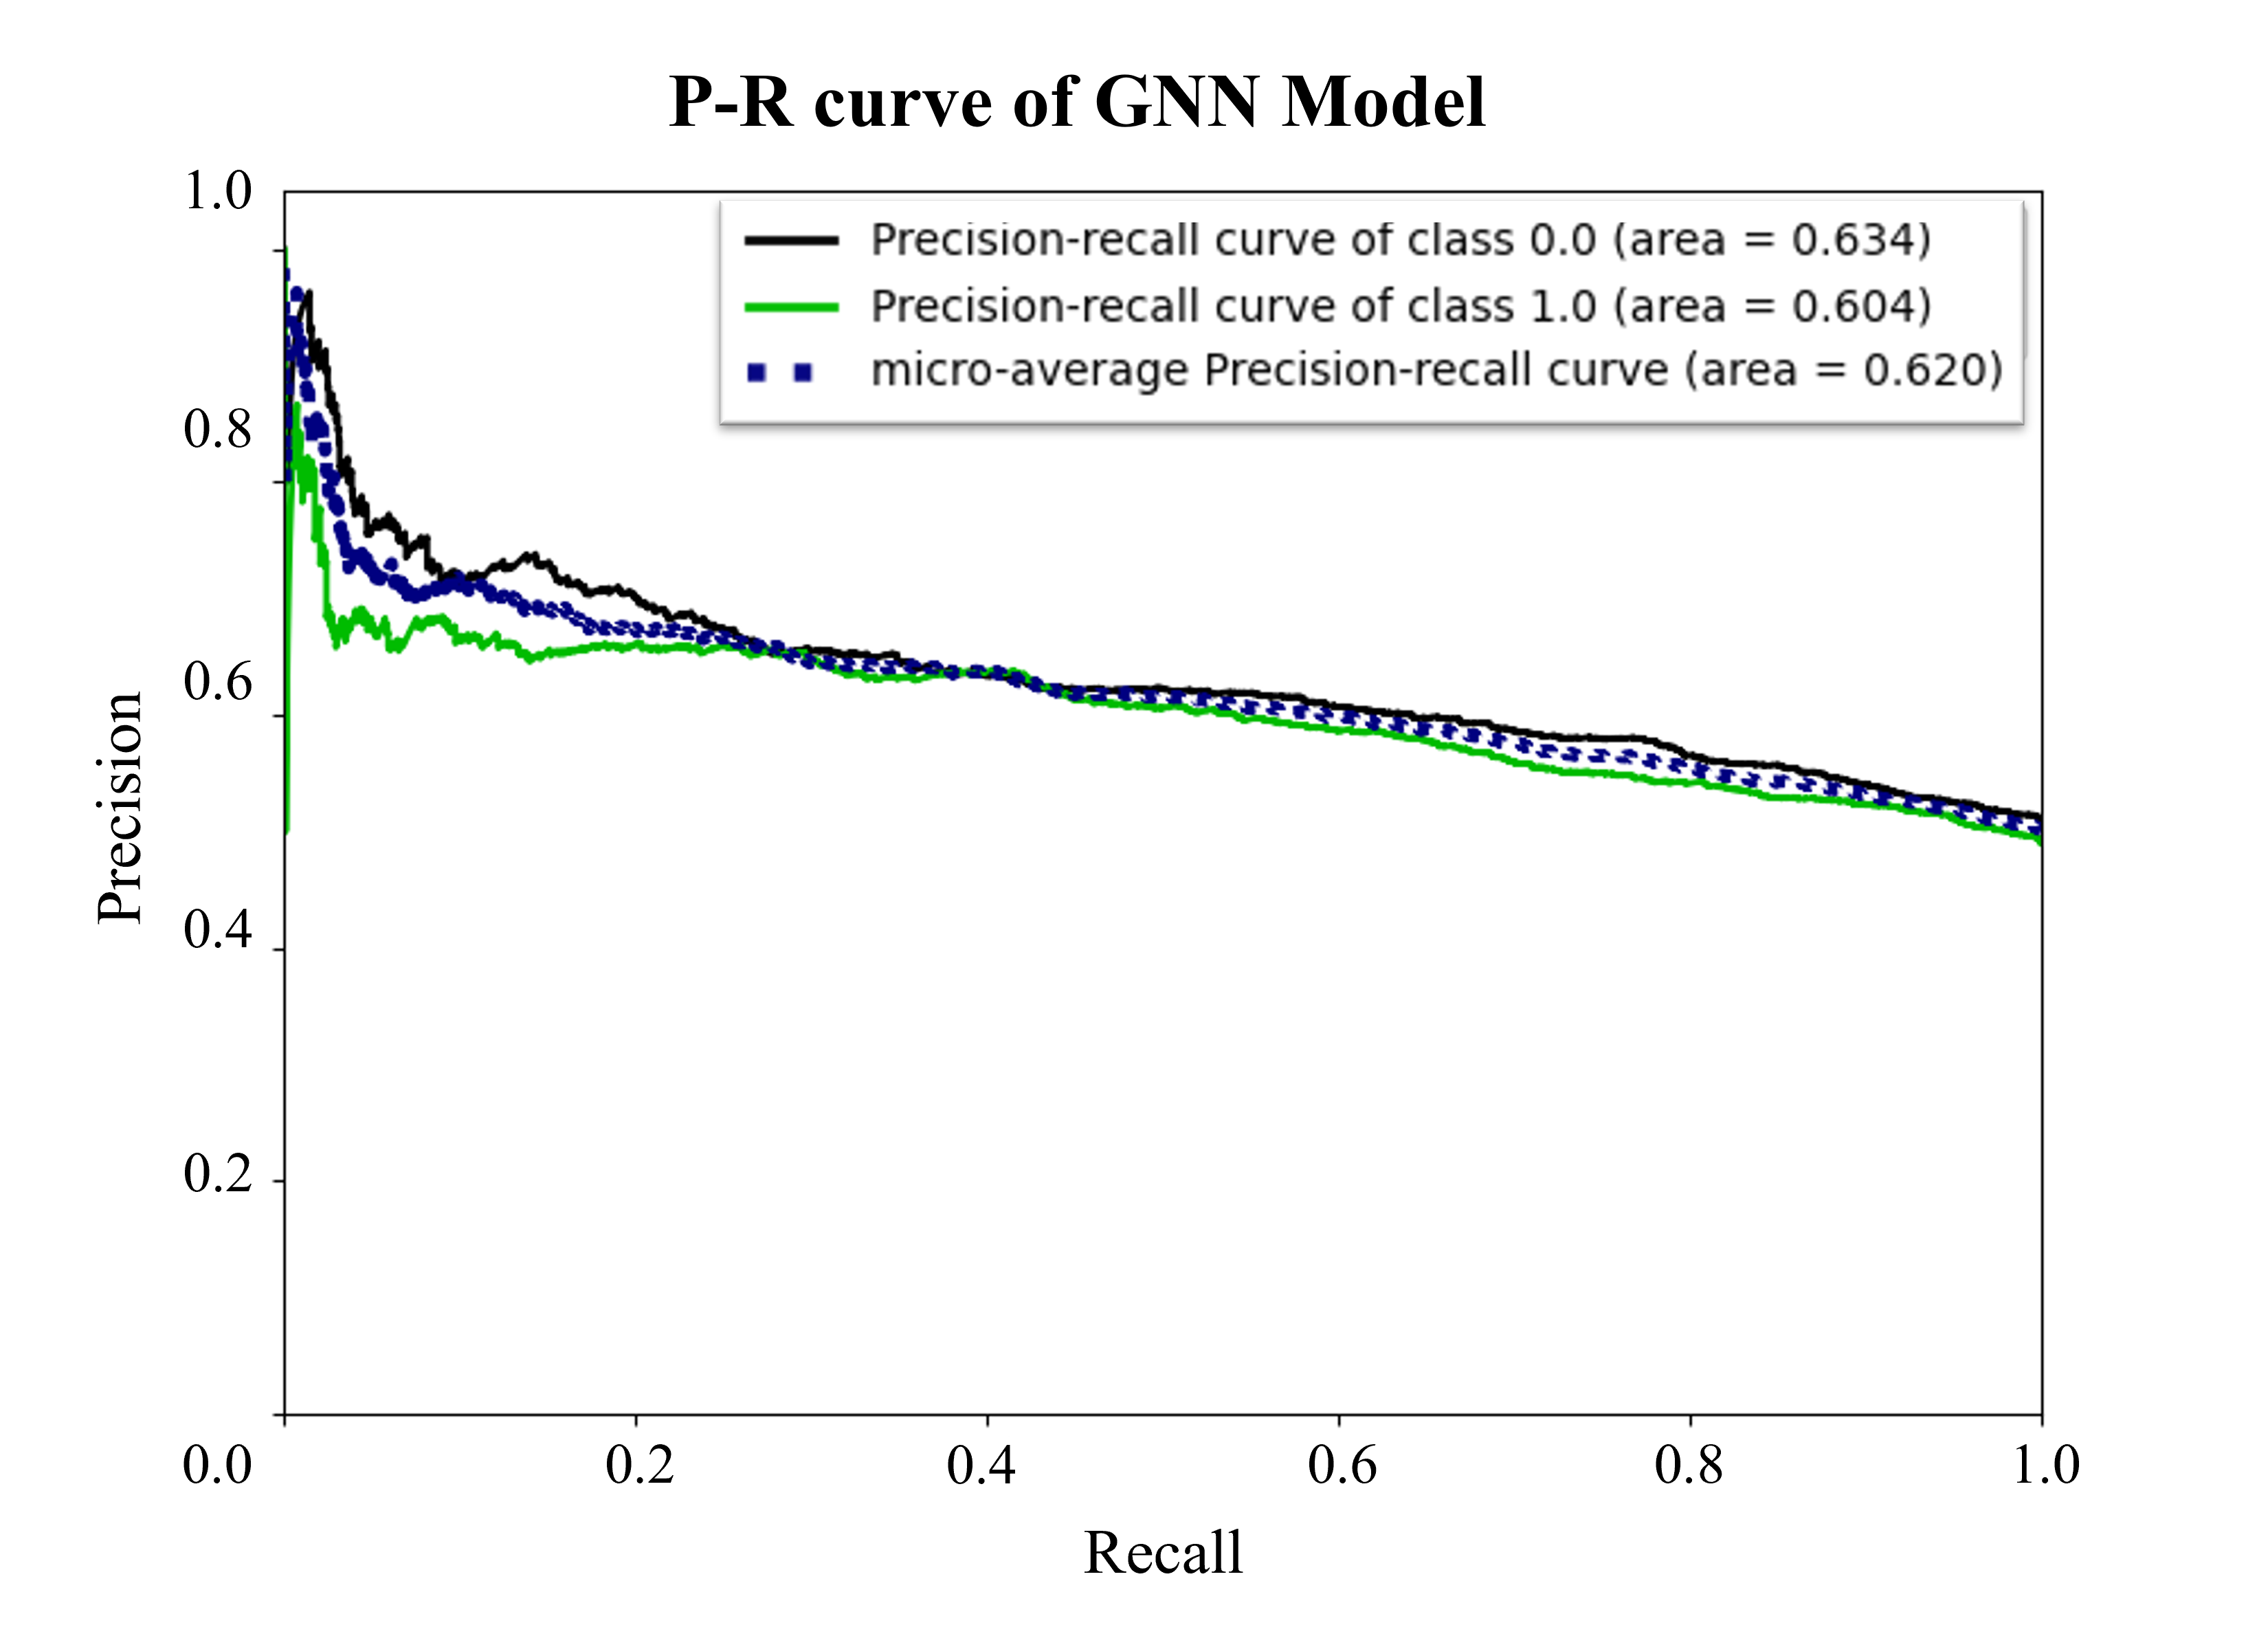
\includegraphics[width=7cm]{figures/Chapter4/GNN/GNNPR.png}
}
\caption{融合表型信息对模型性能的影响}
\end{figure}
可以看出融合表型之后模型性能有了进一步提升。此时预测AUC以及达到0.74,相较于单纯利用基因型数据的图神经网络预测准确能力显著增强。


\section{图估计效果}

\subsection{估计器在训练过程中的效果}

\subsubsection{可行性验证}

为了验证本文设计图估计器对无结构数据的处理能力,在使用该估计器估计本研究所使用骨关节炎患者基因型数据结构之前,本文先在MNIST数据集上进行测试。MNIST数据集\cite{lecun_gradient-based_1998}由若干已标注手写数字图片组成,也是一种无结构数据。我们因此在该数据集上应用我们的模型并将结果加以记录。可以看到,在每个迭代的图估计器工作之后,模型损失有着明显下降,同时分类准确率也有显著提升。这证明了本文提出图估计器对图神经网络在无结构数据上的性能有着明显改善,为后续对骨关节炎患者基因型数据的处理工作提供可行性基础。
\begin{figure}[htbp]
\centering
\subfigure[MNIST数据集上训练损失曲线]{
\includesvg[width=7cm]{figures/Chapter4/EM/MNIST/TrainLoss.svg}
}
\subfigure[MNIST数据集上训练准确率曲线]{
\includesvg[width=7cm]{figures/Chapter4/EM/MNIST/Trainacc.svg}
}
\caption{图估计器在MNIST数据集上的测试结果}
\end{figure}


\subsubsection{对照组}

图估计器的工作过程涉及到图神经网络参数与图结构的循环更新。为了排除多次重启训练对模型性能的潜在影响,我们设计对照组,即使用全连接法构建图矩阵并且每次图神经网络训练之后不更新图结构。并对对照组的模型训练情况做以记录。可以看到,在不更新图结构时,每次迭代中模型损失与准确率的变化趋势基本一致,同时不同迭代末期模型AUC变化不大。因此我们认为模型效果与无图结构更新过程的迭代次数无关
。
\begin{figure}[htbp]
\centering
\subfigure[训练损失曲线]{
\includesvg[width=7cm]{figures/Chapter4/EM/Baseline/TrainLoss.svg}
}
\subfigure[训练准确率曲线]{
\includesvg[width=7cm]{figures/Chapter4/EM/Baseline/Trainacc.svg}
}
\subfigure[测试AUC曲线]{
\includesvg[width=7cm]{figures/Chapter4/EM/Baseline/Valauc.svg}
}
\caption{对照组训练结果}
\end{figure}

\subsubsection{实际数据}

该组试验中我们正式将图估计器与图神经网络运用于骨关节炎患者基因型数据的处理过程中。我们首先使用全连接法构建初始图,在每个迭代中我们训练神经网络并给出数据在该网络下的输出,再将输出作为图估计器的观察值并基于此更新图结构,再将该图结构作为数据的结构重新输入图神经网络中训练。如此迭代若干次,记录模型性能如下。
\begin{figure}[htbp]
\centering
\subfigure[训练损失曲线]{
\includesvg[width=7cm]{figures/Chapter4/EM/Exp/TrainLoss.svg}
}
\subfigure[训练准确率曲线]{
\includesvg[width=7cm]{figures/Chapter4/EM/Exp/Trainacc.svg}
}
\subfigure[测试AUC曲线]{
\includesvg[width=7cm]{figures/Chapter4/EM/Exp/Valauc.svg}
}
\caption{实际数据训练结果}
\end{figure}
可以看出,首次迭代中由于使用全连接网络,模型性能变化同对照组中模型相仿。但是在首次迭代结束生成新图结构后并以此进行第二次迭代的图神经网络训练时我们可以发现,训练末期模型损失明显下降,模型准确率明显上升。模型预测能力AUC也有明显提高。最终我们选择预测能力最好的迭代作为最优模型,参与到骨关节炎风险预测过程之中。

\subsection{图估计器工作过程分析}

\subsubsection{聚类参数选择}

在讨论图估计器时我们提到,图估计器在输入观察值的同时还需要人工选择聚类参数$k$以初始化变分参数,且该聚类参数会对估计结果产生直接影响,该影响可通过整合分类似然评估。为了选择最优聚类参数,我们计算了使用一定范围内的聚类参数时的模型整合分类似然,结果如下。
\begin{figure}[!ht]
\centering
\includesvg[width=\textwidth]{figures/Chapter4/VEM/Model/ModelSelection.svg}
\caption{整合分类似然变化曲线} \label{fig_ch2}
\end{figure}

可以发现,$k$取6时模型的整合分类似然最低,性能最好。同时我们考虑了在使用该范围内参数时变分期望最大化算法所给出的证据下界ELBO,我们发现虽然$k$取6的组证据下界并非最高,但是同其他组相比也处于高位。因此我们将$k$定为6并估计该参数下可能的图结构。

\begin{figure}[!ht]
\centering
\includesvg[width=\textwidth]{figures/Chapter4/VEM/Model/Iteration.svg}
\caption{证据下界曲线} \label{fig_ch2}
\end{figure}


\subsubsection{生成图结构分析}

根据前文对变分期望最大化算法的讨论我们可以发现,$k$取6意味着最终生成的图结构可以分为6簇。为了探究该网络结构以及其潜藏的信息,我们将估计图结构中的节点依照其所属的簇加以归类并表示如下图。

\begin{figure}[!ht]
\centering
\includesvg[width=\textwidth]{figures/Chapter4/VEM/Model/Cluster.svg}
\caption{节点簇信息} \label{fig_ch2}
\end{figure}

我们同时将计算所得的簇与簇之间的关系表示如下。可以发现,簇3与簇4、簇2与簇6之间存在着很强的相关信号。且簇6与除簇1,2之外的其它簇关联都不强。我们同时发现簇3、5之间也存在一相关信号。除此以外数学分析无法从该图中获取更多信息,我们因此需要结合图中节点的生物学意义对该图结构与簇关系加以分析。

\begin{figure}[htbp]
\centering
\subfigure[簇之间关联图]{
\includesvg[width=7cm]{figures/Chapter4/VEM/Model/meso.svg}
}
\subfigure[簇关系邻接矩阵]{
\includesvg[width=7cm]{figures/Chapter4/VEM/Model/NetADJ.svg}
}
\caption{簇之间关系}
\end{figure}

\subsubsection{结合表型分析}

为了进一步探究生成图结构的生物学意义,我们需要了解其中节点,也就是SNP位点对人的不同表型的贡献。同GWAS研究类似的,全表型关联研究(Phenome-wide Association Study,PheWAS)主要研究某一SNP位点与已知性状的关联\cite{pendergrass_use_2011},因此我们对图中每个节点进行PheWAS研究。我们对节点的研究主要在GWASATLAS数据库内进行\cite{watanabe_global_2019},该数据库包含了在UKB数据上进行的对3302个表型的约4756个GWAS研究,可以较为全面地展现SNP位点对表型的影响。对于每个SNP,我们编写爬虫由数据库获取与其相关的表型以及该相关的统计学显著性,经过统计学显著性筛选($p<10^{-5}$)后将与每个SNP相关的表型按照领域分为25类。对于每个簇,我们统计簇内SNP位点对每类性状的关联并进行簇内标准化,得出如下热图。

\begin{figure}[htbp]
\centering
\includesvg[width=\textwidth]{figures/Chapter4/VEM/Cluster/heatmap_col.svg}
\caption{簇与性状关联簇内标准化热图} \label{fig_ch2}
\end{figure}

可以看出,每个簇内与簇内SNP相关联程度最高的表型均集中在代谢与免疫领域,这也与骨关节炎本身炎症性质相关。为了能近一步分析簇间差异,我们还对每个领域内关联进行簇间标准化,得到如下热图。

\begin{figure}[htbp]
\centering
\includesvg[width=\textwidth]{figures/Chapter4/VEM/Cluster/heatmap_row.svg}
\caption{簇与性状关联簇间标准化热} \label{fig_ch2}
\end{figure}

相较于簇内标准化,我们可以从此图中发现簇间的明显差异,尤其是簇1、5在环境、内分泌、免疫等领域同其他簇存在明显差异。本文因此对该两簇进行深入分析

\begin{figure}[htbp]
\centering
\subfigure[簇相关性状分布饼图]{
\includesvg[width=7cm]{figures/Chapter4/VEM/Cluster/Cluster1.svg}
}
\subfigure[簇相关性状分布柱图]{
\includesvg[width=\textwidth]{figures/Chapter4/VEM/Cluster/Cluster1bar.svg}
}
\subfigure[簇相关性状p值图]{
\includesvg[width=\textwidth]{figures/Chapter4/VEM/Cluster/Pvaluesofcluster1.svg}
}
\caption{簇一相关性状分领域图}
\end{figure}

同其他簇相同,与簇一内SNP位点相关表型主要集中在代谢与免疫领域。但是我们从热图中发现簇一有着较强的环境相关信号。我们对该环境相关信号加以统计,结果如表所示。出乎我们意料的是,与簇一内SNP相关的环境相关表型出现了受教育程度、工作是否涉及重体力劳动等看起来与骨关节炎毫不相干的性状。但是,在查阅文献\cite{jensen_hip_2008}后我们了解到,骨关节炎作为一种退化性疾病有可能与关节过度磨损相关。因此我们做出猜测,受教育程度较低的个体趋向于从事体力型劳动,导致关节加速磨损,最终导致骨关节炎的发生。而该簇内的SNP可能在受到这种环境影响时更易导致骨关节炎的发生。我们猜测该簇内SNP可能与环境因素导致关节磨损继而导致的骨关节炎相关。
\begin{table}[!h]
	\renewcommand{\arraystretch}{1.2}
	\centering\wuhao
	\caption{簇一相关表型} \label{ICD_exclude} \vspace{2mm}
	\begin{tabularx}{\textwidth} { 
   >{\centering\arraybackslash}X 
   >{\centering\arraybackslash}X
   >{\centering\arraybackslash}X}
	\toprule[1.5pt]
	领域 & 表型 & 计数 \\
	\midrule[1pt]
Environment & Educational attainment & 10 \\
Environment & Education - Qualifications & 3 \\
Environment & Attendance/disability/mobility allowance: Blue badge &
1 \\
Environment & Job involves heavy manual or physical work & 1 \\
Environment & Maternal smoking around birth & 1 \\
	\bottomrule[1.5pt]
	\end{tabularx}
\end{table}

\begin{figure}[htbp]
\centering
\subfigure[簇相关性状分布饼图]{
\includesvg[width=10cm]{figures/Chapter4/VEM/Cluster/Cluster5.svg}
}
\subfigure[簇相关性状分布柱图]{
\includesvg[width=\textwidth]{figures/Chapter4/VEM/Cluster/Cluster5bar.svg}
}
\subfigure[簇相关性状p值图]{
\includesvg[width=\textwidth]{figures/Chapter4/VEM/Cluster/Pvaluesofcluster5.svg}
}
\caption{簇五相关性状分领域图}
\end{figure}

我们也对簇五进行了类似分析,相较于其他簇,簇五在免疫、内分泌、皮肤病领域有着很强相关。我们对这些领域内的典型性状加以统计得到表。可以看出,簇五内的SNP与二型糖尿病、巨噬细胞、白细胞与粒细胞计数相关表型都存在着相关。二型糖尿病是一种由于机体胰岛素抗性而生成的糖尿病,其主要由超重乃至肥胖而导致。\cite{maruthur_diabetes_2016}而肥胖导致的高血脂又会诱发体内免疫系统包括巨噬细胞与粒细胞的激活。\cite{barrett_diabetes-mediated_2017}这也与簇内的观察一致,因此我们猜测簇五内的SNP位点主要与个体自身肥胖导致的糖尿病与超重继而诱发的自身型骨关节炎相关。

\begin{table}[!h]
	\renewcommand{\arraystretch}{1.2}
	\centering\wuhao
	\caption{簇五相关表型} \label{ICD_exclude} \vspace{2mm}
	\begin{tabularx}{\textwidth} { 
   >{\centering\arraybackslash}X 
   >{\centering\arraybackslash}X
   >{\centering\arraybackslash}X}
	\toprule[1.5pt]
	领域 & 表型 & 计数 \\
	\midrule[1pt]
Endocrine & Type 2 Diabetes & 25 \\
Immunological & Myeloid white cell count (three-way meta) & 14 \\
Immunological & White blood cell count (three-way meta) & 14 \\
Immunological & Granulocyte count (three-way meta) & 13 \\
Dermatological & Male pattern baldness & 10 \\
	\bottomrule[1.5pt]
	\end{tabularx}
\end{table}

以上我们通过对图估计生成图结构的分析将输入的致病SNP分为六簇并对其中两个典型簇进行具体生物学意义分析。同时根据两簇内SNP的相关性状提出了骨关节炎的两种诱因,即由环境因素导致关节过度磨损诱发的骨关节炎以及由于超重诱发的自身型骨关节炎。而这类分析是传统机器学习模型所无法实现的,这也进一步印证了图神经网络在学习数据深度信息时的出众能力。

\section{图解释器结果案例分析}

我们之前提到本风险预测模型中的图解释器能对产生预测结果的原因,即输入基因型图中同预测结果相关的最大子图,加以分析与计算。本节通过模型对UKB数据库中一个案的分析结果展示该能力。本文从UKB数据库中选取样本(UID=5125713),并将其基因型数据根据图估计器给出的最佳图结构转为图数据。利用训练好的图神经网络模型对该图进行处理,预测结果为该样本有很高概率患骨关节炎。我们将该预测结果与模型输入图解释器中,最终图解释器给出如下相关子图。

\begin{figure}[htbp]
\centering
\includesvg[width=\textwidth]{figures/Chapter4/VEM/Explain/Main.svg}
\caption{图解释器生成与预测结果相关子图} \label{fig_ch2}
\end{figure}

在该子图中,边的权重为该关联对预测值的贡献,权重越高代表该边对预测值的生成越“重要”。我们将该图按照边的权重进行稀疏化,得到如下系列子图。可以看到,随着权重阈值的不断提升,子图的骨干逐渐显现,而该主干则主要由簇一、五中的节点构成。上一节的分析中我们提到簇五中所含位点可能与二型糖尿病相关,我们因此推测该个体可能由肥胖造成的关节过度磨损诱发骨关节炎,同时该患者可能合并二型糖尿病。我们从UKB数据库中提取患者其他表型。

\begin{figure}[htbp]
\centering
\subfigure[阈值0.315]{
\includesvg[width=8cm]{figures/Chapter4/VEM/Explain/0.315.svg}
}
\subfigure[阈值0.32]{
\includesvg[width=8cm]{figures/Chapter4/VEM/Explain/0.32.svg}
}
\subfigure[阈值0.325]{
\includesvg[width=8cm]{figures/Chapter4/VEM/Explain/0.325.svg}
}
\subfigure[阈值0.33]{
\includesvg[width=8cm]{figures/Chapter4/VEM/Explain/0.33.svg}
}
\caption{子图阈值化结果}
\end{figure}

\begin{table}[!h]
	\renewcommand{\arraystretch}{1.2}
	\centering\wuhao
	\caption{该个体其他表型} \label{ICD_exclude} \vspace{2mm}
	\begin{tabularx}{\textwidth} { 
   >{\centering\arraybackslash}X 
   >{\centering\arraybackslash}X
   >{\centering\arraybackslash}X}
	\toprule[1.5pt]
	UKB-ID & 表型 & 值 \\
	\midrule[1pt]
31 & 性别 & 男 \\
48 & 腰围 & 113 \\
49 & 胯围 & 121 \\
2443 & 确诊糖尿病 & 是 \\
21001 & BMI & 35.2 \\
23098 & 体重 & 105.5 \\
23099 & 体脂率 & 46.1 \\
	\bottomrule[1.5pt]
	\end{tabularx}
\end{table}

患者实际BMI为35.2,体脂率为46\%,已为肥胖体型,并且合并确诊糖尿病。可以看出,患者实际情况同我们根据图结构以及图解释器做出的解释一致。体现了本文提出模型除高效预测骨关节炎风险之外对疾病分型以辅助治疗的能力。

\section{本章小结}

本章对本文搭建的骨关节炎风险预测模型的预测准确性通过若干指标加以评估并同现有的常见疾病风险预测模型算法进行比较,发现本文搭建模型较传统PRS方法与机器学习算法而言在准确性上有着显著提高,已可作为临床辅助工具参与骨关节炎的早期诊断。本章同时对图估计器的工作过程加以记录与展示,一方面验证了算法的可行性;另一方面也证实了图估计器可以显著改善无结构数据在图神经网络中的表现。为了进一步挖掘潜藏在估计器所得图结构中的信息,本章还结合图估计器输出数学模型与图中节点的PheWAS研究结果对图中的簇聚节点之间关系加以分析并且识别出了两个典型簇,并且根据典型簇内节点信息提出了关节炎的两种诱因。最后本章利用模型解释器进行案例分析,在给出预测结果的同时还利用解释器的结果与识别出的典型簇预测了疾病的分型。以上内容完整展现了本模型作为高效准确可解释骨关节炎风险预测模型的功能与性能。